\documentclass [a4paper]{report}
\usepackage{graphicx,array,natbib,amsmath,bm}
\usepackage{geometry}
\usepackage{soul,color}
\usepackage[pagewise]{lineno}
\usepackage{setspace}
\usepackage{listings}
\usepackage{multirow}

\geometry{ hmargin=2.5cm, vmargin=2.5cm }

% \usepackage[latin1]{inputenc}
 %\usepackage[T1]{fontenc}
 %\usepackage[normalem]{ulem}
% \usepackage[french]{babel}
% \usepackage{verbatim}
% \usepackage{graphicx}

\title{\Huge \emph{\textbf{DIYABC}} \\ 
version 2.0\\
------\\ 
A user-friendly software \\  
for inferring population history  through \\ 
Approximate Bayesian Computations\\
using\\ 
microsatellite, DNA sequence and SNP data}
\vspace{1.0 cm}
\author{
\Large J.M. Cornuet, P. Pudlo,\\ 
\Large J. Veyssier, A. Dehne-Garcia and A. Estoup\\
\vspace{6.0cm}
Centre de Biologie et de Gestion des Populations\\
Institut National de la Recherche Agronomique\\
Campus International de Baillarguet, CS 30016 Montferrier-sur-Lez\\
34988 Saint-G\'ely-du-Fesc Cedex, France\\
\texttt{(diyabc@cbgp.supagro.fr)}}


\date{\today}
\normalsize

% Ce qui suit sert à numéroter les section, sous-sections, ... � partir de 1 au lieu de 0
\setcounter{secnumdepth}{4} 

\renewcommand{\thesection}{\arabic{section}.} 
\renewcommand{\thesubsection}{\thesection \arabic{subsection}} 
\renewcommand{\theparagraph}{\thesubsection.\arabic{paragraph}} 

\let\sectionv\section 
\renewcommand{\section}[1]{\sectionv{#1} \setcounter{paragraph}{0}} 

\let\subsectionv\subsection 
\renewcommand{\subsection}[1]{\subsectionv{#1} \setcounter{paragraph}{0}} 
% Fin de la modif de renum�rotation

\linenumbers
\begin{document}
\maketitle %\clearpage
\pagestyle{myheadings}
\markboth{DIYABC v2.0}{DIYABC v2.0}
\begin{doublespacing}
\setcounter{tocdepth}{4}
\tableofcontents
\end{doublespacing}
\newpage
\section{Preface}
In less than 10 years, Approximate Bayesian Computations (ABC) have developed in the Population Genetics community as a new tool for inference on the past history of populations and species. Compared to other approaches based on the computation of the likelihood which are still restrained to a very narrow range of evolutionary scenarios and mutation models, the ABC approach has demonstrated its ability to stick to biological situations that are much more complex and hence realistic. However, this approach still requires numerous computations to be performed so that it has been used mostly by specialists (i.e. statisticians and programmers). This has almost certainly restrained the possible impact of ABC in population genetic studies. We believe that this situation must be improved and therefore we have developed a computer program for the large community of experimental biologists. We therefore designed $DIYABC$ as a user-friendly program allowing non specialist biologists to achieve their own analysis.\

\textbf{The first version ($DIYABC$ v$0.x$)} had been written especially for microsatellite data. There were at least two reasons for that. The first one is that we have been among the first to develop and use this class of markers in population genetic studies \citep[e.g.][]{E1993}. Since then, we have developed microsatellites in numerous species as well as we have published theoretical studies and reviews on these markers \citep[e.g.][]{E2002}. The second reason is that microsatellites have been and still are very popular markers in the population geneticist community and there is now a large quantity of data that might benefit of an ABC approach.\

\textbf{The second version of our software ($DIYABC$ v$1.x$)} has been designed to make use of DNA sequence data.This has several immediate consequences. For instance, the standard Genepop data file format has been extended to incorporate sequence data. This has been done in collaboration with the authors of $Genepop$ and explained in  subsection 4.1.1. In this version, sequence loci are considered in the same way as microsatellite loci, i.e. they are considered as genetically independent and intra-locus recombination is not (yet) available. Regarding mutation models for DNA sequences, we used the same philosophy as for microsatellites, i.e. the program considers only simple and widely used models, keeping in mind that a higher-dimensional parameter space will be less well explored than a lower-dimensional space. Note that none of these mutation models includes insertion-deletions. 
Also five categories of loci (either microsatellites or DNA sequences) were considered in this second version : autosomal diploid, autosomal haploid, X-linked, Y-linked and mitochondrial. Note that X-linked loci can be used for an haplo-diploid species in which both sexes have been sampled. If non-autosomal loci have been typed in population samples, the sex-ratio of the species will have to be provided (see subsection 4.1.1).\\ 

%Also for DNA sequence loci, one can choose among two possibilities : either each locus has its own mutation model or they all share the same mutation model (but not the same mutation parameters). Going back to microsatellites, there is an additional mutation parameter added to this version : the mean rate of single nucleotide insertion-deletion mutations.\\

%Given that mitochondrial DNA sequences are commonly used by population geneticists and that different effective population sizes correspond to such monoparental loci, a specific code has also been added to the genepop format to comply with this new requirement (see 4.1.1 for details). 

Other improvements over version 0 included :
\begin{enumerate}
\item the use of multithread technology in order to exploit multicore/multiprocessor computers. This is especially useful when building the reference table and for several other intensive computation steps, such as the multinomial logistic regression,
\item a new option which helps the detection of "bad" prior modelisation of the data, 
\item another new option which helps evaluate the goodness of fit of a given model-parameter posterior combination (i.e. Model checking),   
\item many new screens implemented not only to treat sequence data, but also to cope with the new options described above, as well as to offer useful complementary information on the current run. 

\end{enumerate}

 \textbf{The third version of $DIYABC$ ($DIYABC$ v$2.x$)}  has been entirely recoded in order to be used under the usual three OS (Linux, Windows and Mac). Also the code for computations has been separated from that of the graphic user interface (GUI). The former has been rewritten in C++ and the latter is a mixture of Python and Qt (PyQt). The user can then launch computations with or without using the GUI. The GUI 's uses are : 

\begin{enumerate}
\item the management of projects
\item the input of the historical and genetical models
\item the parameterization of analyses
\item the launch of computations  of the reference table and of the various required analyses
\item the visualization of results
\end{enumerate}

We recommend non-expert users to use the GUI for their computations.\\

Also, as DNA sequences have been added in the second version, a new category of markers has been added to the third version : Single Nucleotide Polymorphisms (SNPs). Instead of extending once more the Genepop format, a new data simple format has been designed for these markers. Note that SNP data are treated separately from other markers ($i.e.$ they cannot be analyzed together with microsatellite and/or DNA sequence data).\\  

This version includes all improvements of version 1.x and a few new improvements such as :
\begin{itemize}
\item loci of the same type (i.e. microsatellites on one hand or DNA sequences on the other hand) can be associated in one or more groups. This allows for instance to define different mutation models for microsatellites with motifs of different lengths.
\item  the model checking option is now presented as a direct option (not a suboption of the ABC estimation of parameters) which largely simplifies its use.
\item the logistic regression can be performed on linear discriminant analysis components instead of all summary statistics. This reduces the number of dependent variables, thus allowing to run large "confidence in scenario choice" analyses including many summary statistics and scenarios \citep{EL2012}.
%\item ascertainment bias in the design of SNPs can be tentatively corrected by considering ``reference'' samples in which the loci need to be polymorphic in order to belong to the SNP set. These reference samples are not necessarily included of the actual samples.
\end{itemize}

\subsection{Acknowledgements}
We thank Mark Beaumont who has been at the origin of our interest for ABC. He offered us constant help and inspiration since the beginning. We also thank David Balding who welcomed one of us (JMC) in his team during the whole writing of the program and who organized several workshops on ABC during the same period. We are indebted to Christian Robert, Jean-Michel Marin, Stuart Baird, Thomas Guillemaud, Renaud Vitalis, Gael Kergoat, Gilles Guillot and David Welsh with whom we discussed many theoretical and practical aspect of DIYABC in the numerous meetings financed by a grant from the French Research National Agency (project $MISGEPOP$ ANR-05-BLAN-196). The same grant is also aknowledged for having paid for the 2-year salary of FS. This research was also supported by an EU grant awarded to JMC as an EIF Marie-Curie fellowship (project $StatInfPopGen$) and which allowed him to come to David Balding's place at Imperial College (London, UK). Current and future developments of DIYABC are financed by a new grant from the French Research National Agency (project $EMILE$ ANR-09-BLAN-0145) awarded in september 2009. We thank several “beta-users”, especially Eric Lombaert, Christophe Plantamp, Marie-Pierre Chapuis, Carine Brouat and Michael Fontaine, who tested the the DIYABC V2 software with their data.
\subsection{References to cite}
\begin{itemize}
\item \textbf{version 0 :} Cornuet J.M., F. Santos, M.A. Beaumont, C.P. Robert, J.M. Marin, D.J. Balding, T. Guillemaud and A. Estoup. Inferring population history with DIYABC: a user-friendly approach to Approximate Bayesian Computations (2008) \emph{Bioinformatics}, \textbf{24} (23), 2713-2719.
\item  \textbf{version 1 :}  Cornuet J.M., V. Ravign\'e and A. Estoup, 2010. Inference on population history and model checking using DNA sequence and microsatellite data with the sofware DIYABC (v1.0) (2010) \emph{BMC Bioinformatics}, \textbf{11}, 401.
\item  \textbf{version 2 :}  Cornuet J.M., Veyssier J., Pudlo P., Dehne-Garcia A., Gautier M., Leblois R., J.M. Marin and A. Estoup. $DIYABC$ v2.0: a software to make Approximate Bayesian Computation inferences about population history using Single Nucleotide Polymorphism, DNA sequence and microsatellite data. \emph{submitted}
\end{itemize}
\subsection{Web site}
http://www1.montpellier.inra.fr/CBGP/diyabc\\



\newpage
\section{Methodology}
\subsection{Basic notions on ABC} Approximate Bayesian Computation or
ABC is a bayesian approach in which the posterior distributions of
the model parameters are determined by replacing the computation of
the likelihood (probability of observed data given the values of the
model parameters) by a measure of similarity between observed and
simulated data. The posterior distributions are estimated from
parameter values providing simulated data that are the most similar
to observed data. Historically, different ways of estimating this
similarity have been proposed, but all have been based on statistics
summarizing information conveyed by the data set. In population
genetics, data most often relate to individuals that have been
genotyped at a given set of loci, these individuals being representative of the
studied populations. The summary statistics are for instance the mean
number of alleles per population or genetic distances between pairs
of populations. It is much easier to measure the
similarity between small sets of summary statistics than between
large sets of multilocus genotype data. When the number of summary
statistics is low, it is possible to select simulated data for which
\emph{all} the summary statistics are close to those of the observed
data \citep{P1999,E2001,EC2003}. However, for more complex scenarios
necessitating a larger number of summary statistics, it becomes
almost impossible to find such simulated data sets. \citet{B2002}
have hence proposed to measure similarity through the Euclidian
distance between observed and simulated summary statistics, after normalization by standard
deviations of simulated statistics. In addition, these authors introduced a
step of local linear regression aimed at favoring simulated data
sets that are closer to the observed one.\\
 In practice, the ABC approach can be summarized in three successive
 steps \citep{Ex2005} : i) generating simulated data sets, ii)
 selecting simulated data sets closest to observed data set and iii)
 estimating posterior distributions of parameters through a local
 linear regression procedure.\\ 
 In addition, this approach provides a way of comparing different
 scenarios that can explain observed data. Two measures of posterior probabilities of scenarios are proposed. The first measure is simply the relative proportion of each scenario in the simulated data sets closest to observed data sets \citep{ME2005,PC2007}. The second measure  is obtained by a logistic regression of each scenario probability on the deviations between simulated and observed summary statistics \citep{FR2007,B2008}. \\
 
 
 In order to simulate data, one has first to define one (or possibly
several) model(s). Each model includes a historical model describing
how the sampled populations  are connected to their common ancestor
and a mutational model describing how allelic states of the studied
genes are changing along their genealogical trees.\\

\subsection{Historical model parameterization}
The evolutionary scenario, which is quantified by the historical
model, can be described as a succession in time of "events" and
"inter event periods". The events considered in the program are a
restricted set of possible events affecting populations evolution.
In the current version of the program, we consider only 4 categories
of events : population divergence, 
discrete change of effective population size, admixture and sampling (the last one has been added
to allow considering samples taken at different times). Between two successive
events affecting a population, we assume that populations evolve
independently (e.g. without migration) and with a fixed effective
size. The usual parameters of the historical model are the times of
occurrence of the various events (counted in generations), the
effective sizes of populations and the admixture rates. When writing
the scenario, events are provided sequentially backward in time.
Although this choice may not be natural at first sight, it is coherent with
coalescence theory on which are based all data simulations in the
program. For that reason, the keywords for a divergence or an
admixture event are \texttt{merge} and \texttt{split}, respectively.
Two other keywords, \texttt{varNe} and \texttt{sample},
correspond to a discrete change in effective population size and a gene
sampling, respectively. Eventually, only for SNPs, we have added the keyword \texttt{refsample} to control the ascertainment bias (see below).\\
A scenario takes the form of a succession of lines (one line per
event), each line starting with the time of the event, then the
nature of the event, and ending with several other data depending on
the nature of the event. Following is the syntax used for each
category of event :
\begin{description}
\item[population sample] : $\langle time \rangle$ \texttt{sample} $\langle pop \rangle$  $[nmales$   $nfemales]$  \\ 
$\langle time \rangle$ is the time (always counted in number of generations) at which the sample was taken and\\
 $\langle pop \rangle$ is the population number from which is taken the sample. It is worth stressing here that \textbf{samples are considered
in the same order as they appear in the data file}.\\
$[nmales$   $nfemales]$ is only used for SNP loci to indicate the number of males (respectively females) from the sample that have been used to detect SNPs. Thes males and females appear in the corresponding sample of the data file.
 
\item[``reference'' sample] : $\langle time \rangle$ \texttt{refsample} $\langle pop \rangle$  $nmales$   $nfemales$  \textbf{ONLY FOR SNP loci}\\ 
$\langle time \rangle$ is the time (always counted in number of generations) at which the ``reference'' sample was taken and\\
 $\langle pop \rangle$ is the population number from which is taken the sample.\\
$nmales$   $nfemales$ indicate the number of males (respectively females) that have been used to detect SNPs in the reference sample. These males and females \textbf{do not appear} in the data file.

\item[population size variation] : $\langle time \rangle$ \texttt{varNe}
 $\langle pop \rangle$ $\langle Ne \rangle$\\
 From time $\langle time \rangle$, looking backward in time,
 population $\langle pop \rangle$ will have an effective size $\langle Ne
 \rangle$.
\item[population divergence] :
$\langle time \rangle$ \texttt{merge} $\langle pop0 \rangle$
$\langle pop1 \rangle$\\
At time $\langle time \rangle$, looking backward in time, population
$\langle pop1 \rangle$ "merges" with population $\langle pop0
\rangle$. Hereafter, only $\langle pop0 \rangle$ "survives".
\item[population admixture] :
$\langle time \rangle$ \texttt{split} $\langle pop0 \rangle$
$\langle pop1 \rangle$ $\langle pop2 \rangle$ $\langle rate \rangle$\\
At time $\langle time \rangle$, looking backward in time, population
$\langle pop0 \rangle$ "splits" between populations $\langle pop1
\rangle$ and $\langle pop2 \rangle$. A gene lineage from population
$\langle pop0 \rangle$ joins population $\langle pop1 \rangle$
(respectively $\langle pop2 \rangle$) with probability $\langle rate
\rangle$ (respectively 1-$\langle rate \rangle$).
\end{description}

A scenario is a succession of lines as described above. However, in
order to cope with special situations (see explanations in Note
 9 below), we added a first line giving the effective sizes of sampled
populations before the first event described, looking backward in time.
Expressions between arrows, other than population numbers, can be
either a numeric value (e.g. 25) or a character string (e.g.
\texttt{t0}). In the latter case, it is considered as a parameter of
the model. So the only possible parameters of the historical model
are times of events, effective population sizes and admixture
rates.\\
The program offers the possibility to add or remove scenarios, by just clicking on the corresponding buttons. The usual shortcuts (CTRL+C, CTRL+V and CTRL+X) can be used to edit the different scenarios. Some or all parameters can be in common among scenarios.\\

\textbf{Notes}
\begin{enumerate}
\item There are two ways of giving a fixed value to effective population sizes, times and admixture rates. Either the fixed value appears as a numeric value in the scenario windows or it  is given as a string value like any parameter. In the latter case, one gives this parameter a fixed value by choosing a Unifom distribution and setting the minimum and maximum to that value in the prior setting (see section 2.4).
\item All expressions must be separated by at least one space.
\item All expressions relative to parameters can include sums or
differences. For instance, it is possible to write :\\
\texttt{t0 merge 2 3}\\
\texttt{t0+t1 merge 1 2}\\
This means that \texttt{t1} is the time elapsed between the two
events. By imposing \texttt{t1>0} (as explained in section
\textbf{prior and posterior distributions}), this implies that the
divergence of populations 1 and 2 is always more ancient than the
divergence of populations 2 and 3. \
However, one cannot mix a parameter and a numeric value (e.g. \texttt{t1+150} will result in an error). This can be done by writing \texttt{t1+t2} and fixing \texttt{t2} by choosing a uniform distribution with lower and upper bounds both equal to 150. 
\item Time is always given in generations. Since we look backward,
time increases towards past.
\item Negative times are allowed (e.g. the example given in section 3), but not recommended.
\item Population numbers must be consecutive natural integers
starting at 1. The number of population can exceed the number of
samples and vice versa : in other words, unsampled populations can be considered in
the scenario on one hand, and the same population can be sampled
more than once on the other hand.
\item Multi-furcating population trees can be considered, by writing
several divergence events occurring at the same time. However, one
has to be careful to the order of the \texttt{merge} events. For
instance, the following piece of scenario will fail :\\
\texttt{100 merge 1 2} \\
\texttt{100 merge 2 3} \\
This is because, after the first line, population 2, which has
merged with population 1, does not "exist" anymore (the surviving population is population 1). So, it cannot
receive lineages of population 3 as it should as a result of the
second line. The correct ways are either to put line 2 before line
1, or to change line 2 to :\\ \texttt{100 merge 1 3}.
\item Since times of events can be parameters, the order of events
can change according to the values taken by the time parameters. In
any case, before simulating a data set, the program sorts out events
by increasing times \footnote{ Sorting events by increasing times can only be done when all time values are known, i.e. when simulating datasets. When checking scenarios, all time values are not yet defined, so that when visualizing a scenario, events are represented in the same order as they appear in the window used to define the scenario.}. If two or more events occur at the same time,
the order is that of the scenario as it is written by the the user.
\item Most scenarios begin with sampling events. We then need to
know the effective size of the populations to perform the simulation
of coalescences until the next event concerning each population. One
way would have been to provide the population size on the same line
of the scenario description. However, in some scenarios with varying
population sizes, it can not be determined what is the effective
size at the sampling time before the set of time parameter values is
generated. For that reason, we decided to provide the effective size
and the sampling description on two distinct lines.
\end{enumerate}

\textbf{Examples} Below are some usual scenarios with increasing complexity. Each scenario is coded on the left side and a graphic representation given by $DIYABC$ is printed on the right side
\begin{enumerate}
\item One population from which several samples have been taken at
various generations : 0, 3 and 10. The only unknown parameter of the scenario\footnote{Of course, there are also one or more parameter(s) for the mutation model.} is the
 effective population size. \\
\begin{center} 
\begin{tabular}{cc}
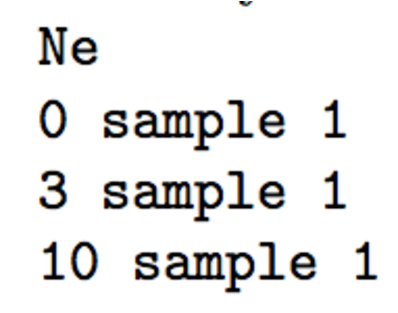
\includegraphics[scale=0.5]{code_scenario_01.pdf} & 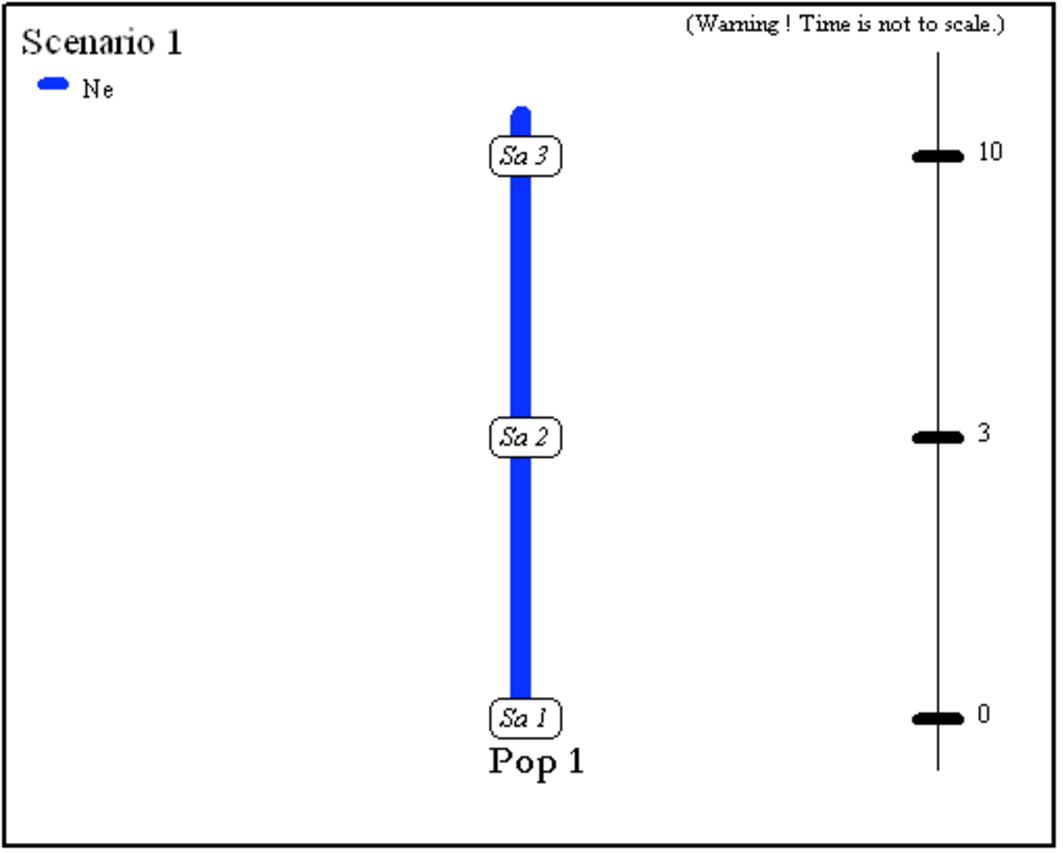
\includegraphics[scale=0.35]{scenario_01.pdf} \\
\end{tabular}
\end{center}

\item Two populations of size \texttt{N1} and \texttt{N2} have diverged \texttt{t} generations
in the past from an ancestral population of size \texttt{N1+N2}.\\
\begin{center} 
\begin{tabular}{cc}
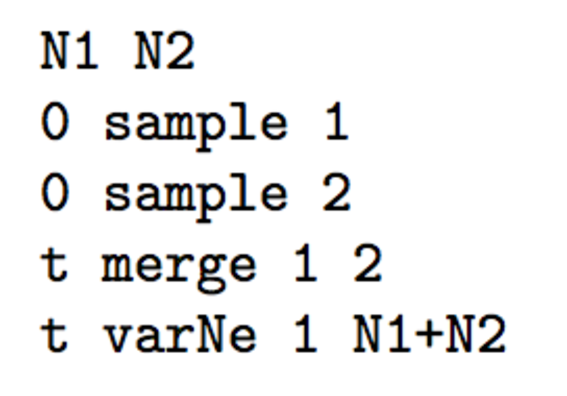
\includegraphics[scale=0.5]{code_scenario_02.pdf} & 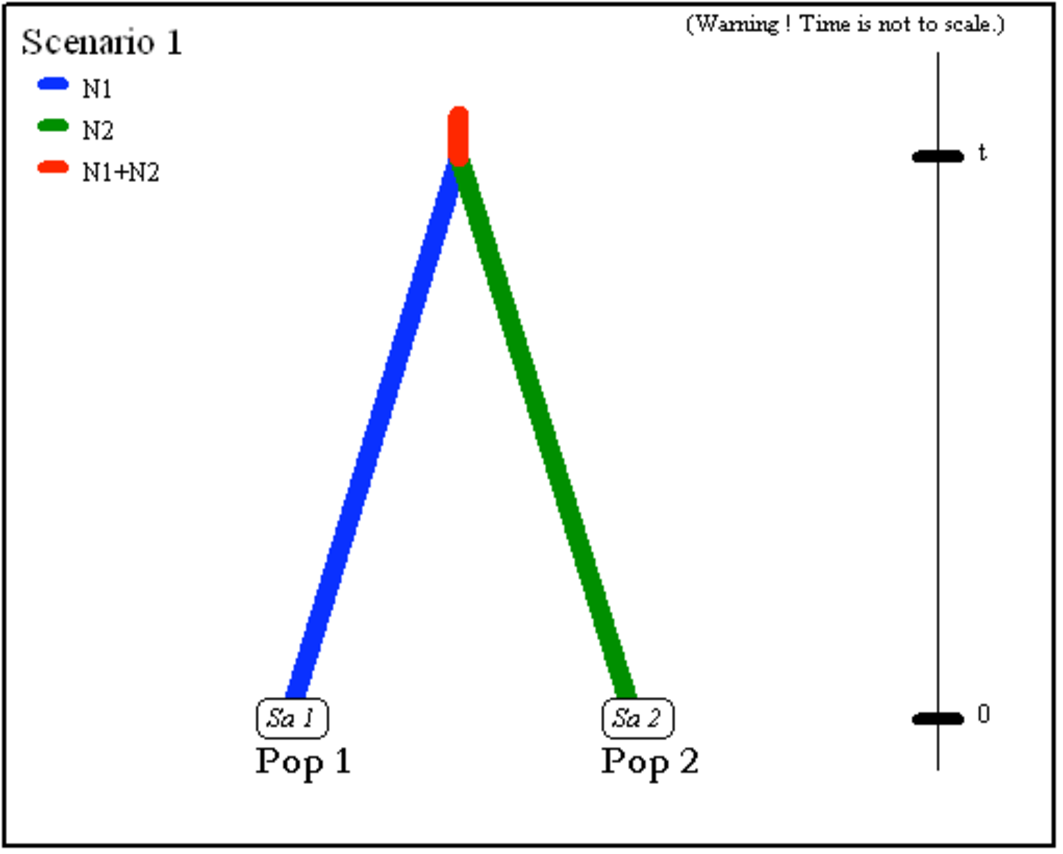
\includegraphics[scale=0.35]{scenario_02.pdf} \\
\end{tabular}
\end{center}


\item Two parental populations (1 and 2) with constant effective populations sizes
\texttt{N1} and \texttt{N2} have diverged at time \texttt{td} from
an ancestral population of size \texttt{NA}. At time \texttt{ta},
there has been an admixture event between the two populations giving
birth to an admixed population (3) with effective size \texttt{N3}
and with an admixture rate \texttt{ra} relative to population 1.\\
\begin{center} 
\begin{tabular}{cc}
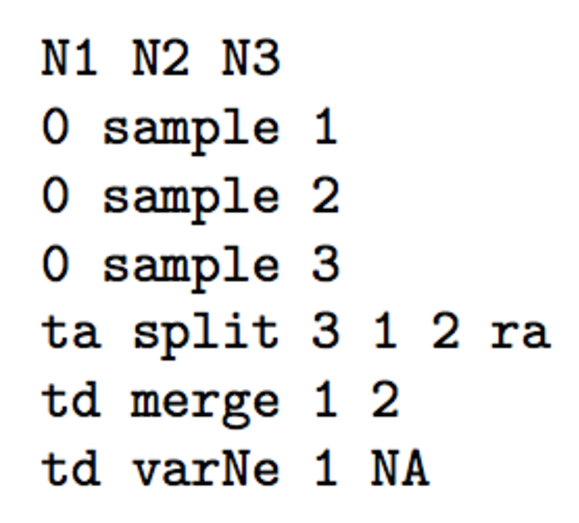
\includegraphics[scale=0.5]{code_scenario_03.pdf} & 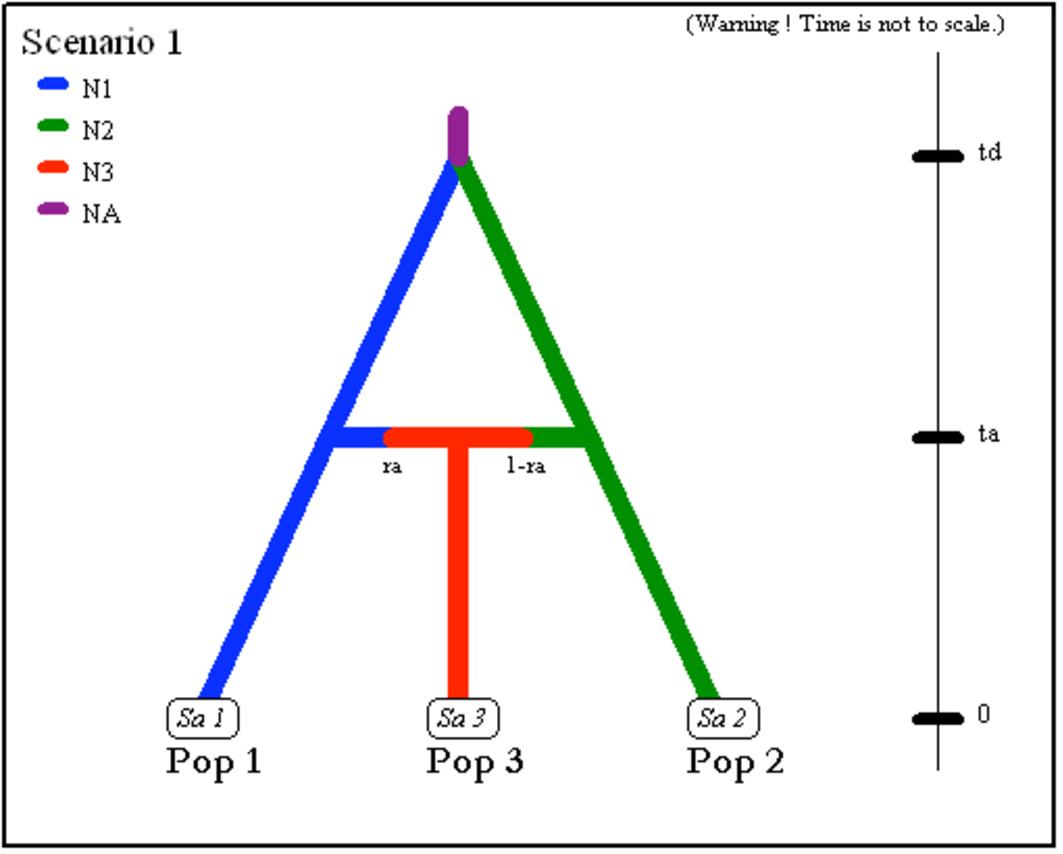
\includegraphics[scale=0.35]{scenario_03.pdf} \\
\end{tabular}
\end{center}

\item The next scenario is slightly more complicated. It includes four population samples and two admixture events.
For simplicity sake, all populations are assumed to have identical effective sizes (\texttt{Ne}).\\
\begin{center} 
\begin{tabular}{cc}
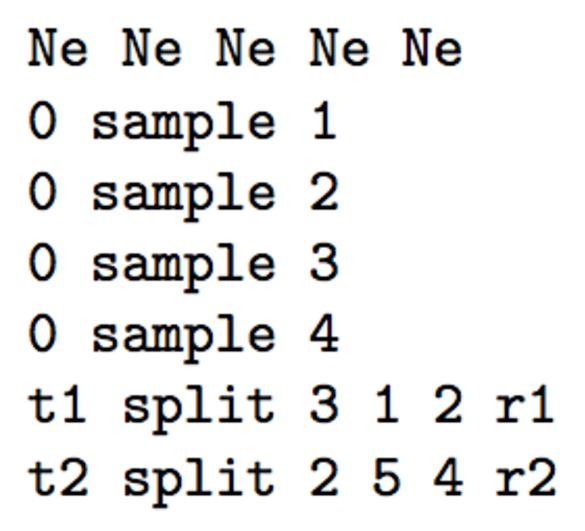
\includegraphics[scale=0.5]{code_scenario_04.pdf} & 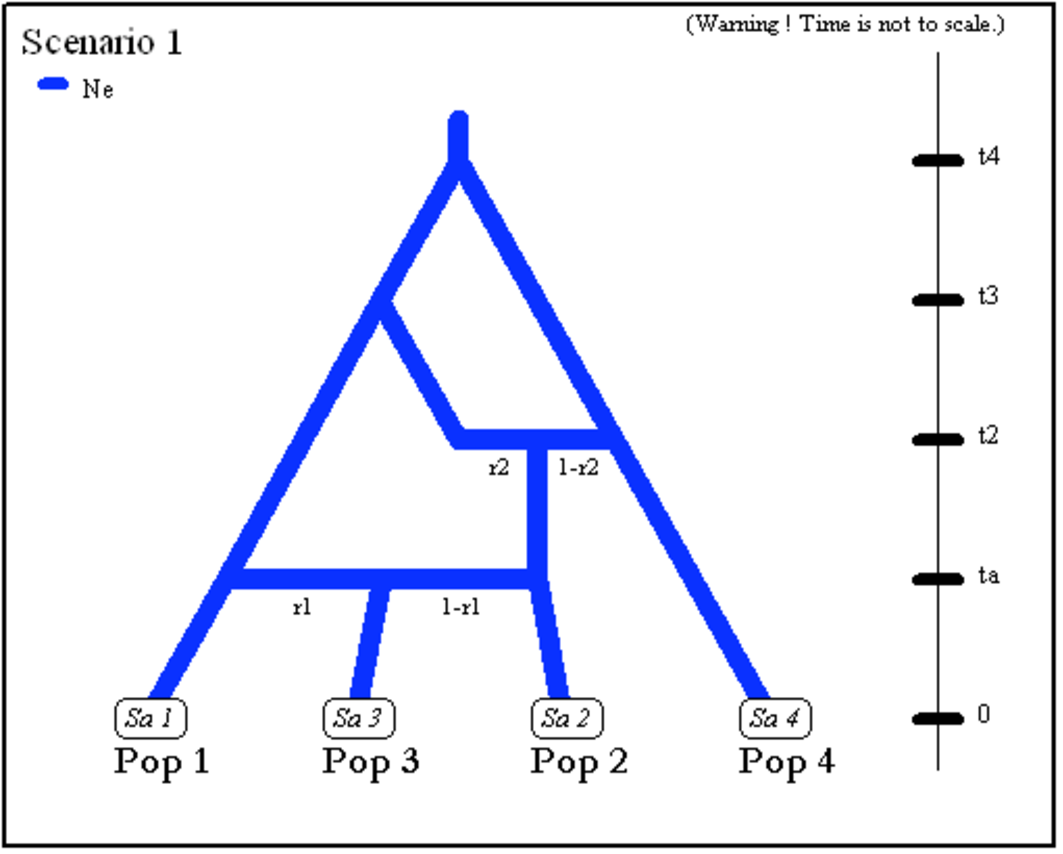
\includegraphics[scale=0.35]{scenario_04.pdf} \\
\end{tabular}
\end{center}



Note that although there are only four samples, the scenario
includes a fifth population. This population which diverged from
population 1 at time \texttt{t3} was a parent in the admixture event
occurring at  time \texttt{t2}. Note also that the first line must include the effective sizes of the \emph{five} populations.\\

\item The following three scenarii correspond to a classic invasion history from an ancestral population (population 1). In scenario 1, population 3 is derived from population 2, itself derived from population 1. In scenario 2, population 2 derived from population 3, itself derived from population 1. In scenario 3, both populations 2 and 3 derived independently from population 1. The same trio of scenarii will be taken later in a fully described example.
Note that when a new population is created from its ancestral population, there is an initial size reduction (noted here \texttt{N2b} for population 2 and  \texttt{N3b} for population 3) since the invasive population generally starts with a few immigrants. 
\end{enumerate}
\medskip \ \ \ \ \ \ \ \  Scenario 1
\begin{center} 
\begin{tabular}{cc}
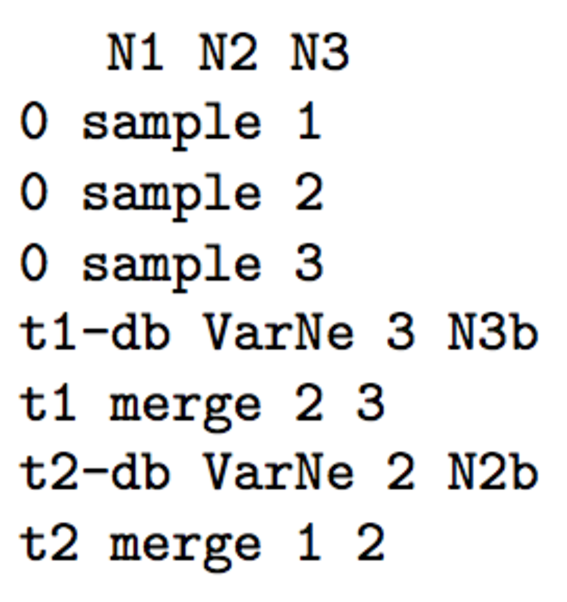
\includegraphics[scale=0.5]{code_scenario_05-1.pdf} & 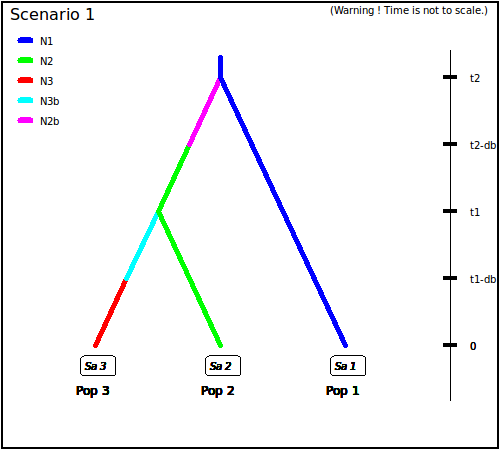
\includegraphics[scale=0.4]{test3pop_scenario_1.png} \\
\end{tabular}
\end{center}

 \ \ \ \ \ \ \ \  Scenario 2
\begin{center} 
\begin{tabular}{cc}
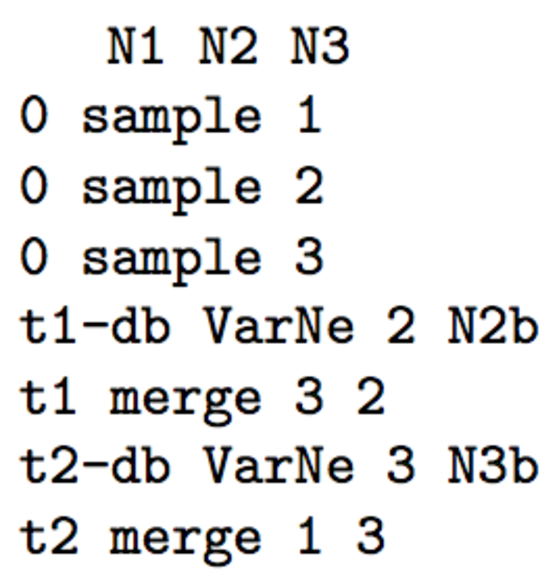
\includegraphics[scale=0.5]{code_scenario_05-2.pdf} & 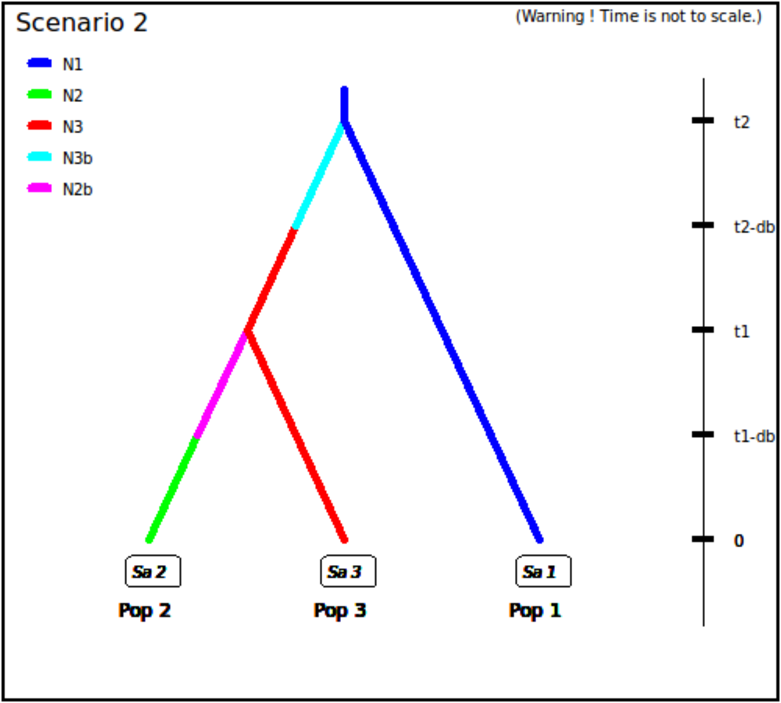
\includegraphics[scale=0.4]{test3pop_scenario_2.pdf} \\
\end{tabular}
\end{center}

\medskip \ \ \ \ \ \ \ \  Scenario 3
\begin{center} 
\begin{tabular}{cc}
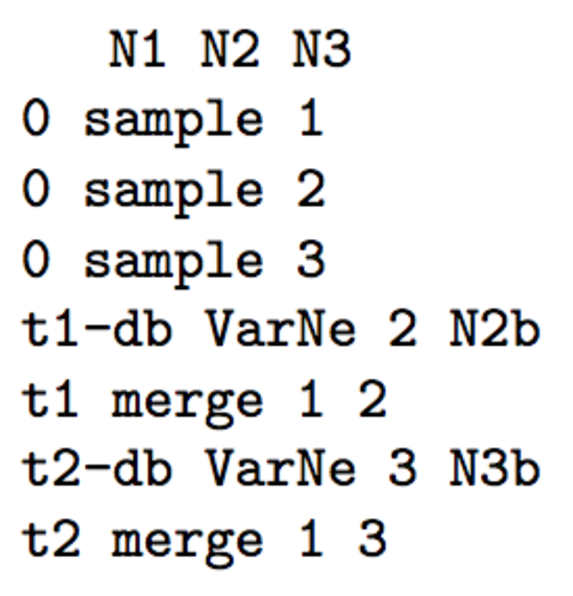
\includegraphics[scale=0.5]{code_scenario_05-3.pdf} & 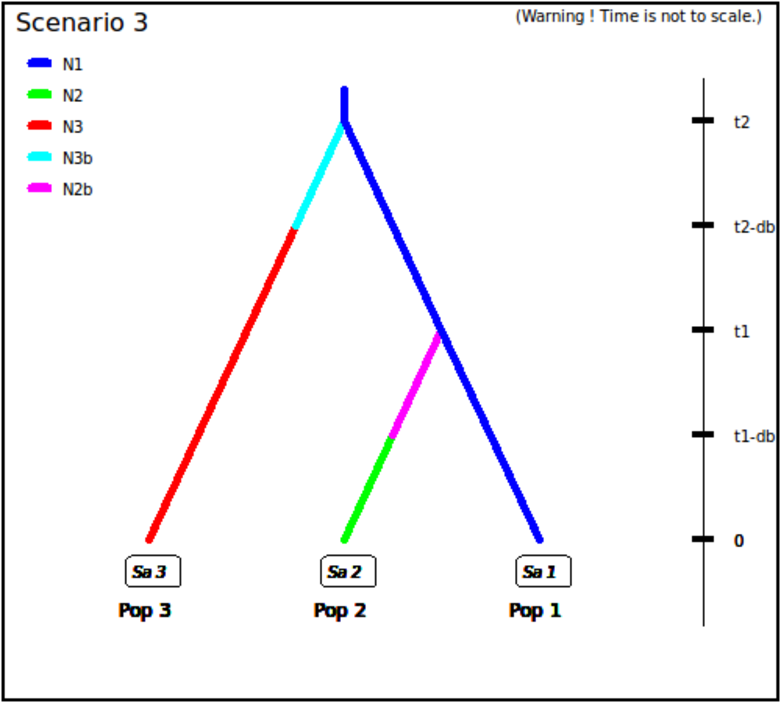
\includegraphics[scale=0.4]{test3pop_scenario_3.pdf} \\
\end{tabular}
\end{center}


\newpage
\subsection{Mutation model parameterization (microsatellite and DNA sequence loci)}
The program can analyse microsatellite data and DNA sequence data altogether as well as separately. In the current version, there  are still two restrictions. First, all loci in an analysis must be genetically independent. Second, for DNA sequence loci, intralocus recombination is not considered.\\

Loci are grouped by the user according to its needs (this an improvement of the current version which imposed all loci of a given category to follow the same mutation model). A different mutation model can be defined for each group. For instance, one group can include all microsatellites with motifs that are 2 bp long and another group those with a 4 bp long motif. Also, with DNA sequence loci, nuclear loci can be grouped together and a mitochondrial locus form a separate group.\\ 
 
The parameterization of the two categories of markers is now described below. 

\subsubsection{Microsatellite loci}
 Although a variety of mutation models have been
proposed for microsatellite loci \citep{W2003}, it is usually
sufficient to consider only the simplest models \citep{C2006}. This
has the non-negligible advantage of reducing the number of parameters, which
can be a real issue when complex scenarios are considered. This is why we chose the Generalized Stepwise Mutation model \citep{E2002}. Under this model, a mutation increases or decreases the length of the microsatellite by a number of repeated motifs  following a geometric
distribution. This model necessitates only two parameters : the mutation rate  (\texttt{$\mu$}) and the parameter of the
geometric distribution (\texttt{$P$}). The same mutation model is imposed to all loci of a given group. However, each locus has its own parameters   (\texttt{$\mu_i$} and \texttt{$P_i$}) and, following a hierarchical scheme, each locus parameter is drawn from a gamma distribution with mean the mean parameter. Note also that :
\begin{enumerate}
\item individual loci parameters (\texttt{$\mu_i$} and \texttt{$P_i$}) are considered as nuisance parameters and hence are never recorded. Only mean parameters are recorded.
\item The variance or shape parameter of the gamma distributions are set by the user and are NOT considered as parameters.
\item The SMM or Stepwise Mutation Model is a special case of the GSM in which the number of repeats involved in a mutation is always one. Such a model can be easily achieved by setting the maximum value of mean P ($\bar{P}$) to 0. In this case, all loci have their $P_i$ set equal to 0 whatever the shape of the gamma distribution.
\item All loci can be given the same value of a parameter by setting the shape of the corresponding gamma distribution to 0 (this is NOT a limiting case of the gamma, but only a way of telling the program). 
\end{enumerate}
Eventually, to give more flexibility to the mutation model, the program offers the possibility to consider mutations that insert or delete a single nucleotide to the microsatellite sequence.  
In the previous version, this option was considered as marginal, and was not treated in the same way as the motif size stepwise mutational process, i.e. there was no associated parameter that could be adjusted to the data. This has been changed in this version :  it is now possible to use a mean parameter (named $ \mu_{(SNI)}$) with a prior to be defined and individual loci having either values identical to the mean parameter or drawn from a Gamma distribution.

\subsubsection{DNA sequence loci}

Note first that this version of the program does not consider insertion-deletion mutations, mainly because there does not seem to be much consensus on this topic. Concerning substitutions, only the simplest models are considered. We chose the Jukes-Cantor (1969) one parameter model, the Kimura (1980) two parameter model, the Hasegawa-Kishino-Yano (1985) and the Tamura-Nei (1993) models. The last two models include the ratios of each nucleotide  as parameters. However, in order to reduce the number of parameters, these ratios have been fixed to the values calculated from the observed data set for each DNA sequence locus. Consequently, this leaves two and three parameters for the Hasegawa-Kishino-Yano (HKY) and Tamura-Nei (TN), respectively.
Also, two adjustments are possible : one can fix the fraction of constant sites (those that cannot mutate) on the one hand and the shape of the Gamma distribution of mutations among sites on the other hand.\\
As for microsatellites, all sequence loci of the same group are given the same mutation model with mean parameter(s) drawn from priors and each locus has its own parameter(s) drawn from a Gamma distribution (same hierarchical scheme). Notes 1, 2 and 4 of previous subsection (2.3.1) apply also for sequence loci.

\subsection{SNPs do not require mutation model parameterization}

SNPs have two characteristics that allow to get rid of mutation models : they are polymorphic and they present only two allelic (ancestral and derived) states. In order to be sure that all analyzed SNP loci have the two characteristics, non polymorphic loci are disgarded right from the beginning of analyses. Consequently, no matter \emph{how} it occurred, we can assume that there occured one and only one mutation in the coalescence tree of sampled genes. We will see below that this  largely simplifies (and speeds up) SNP data simulation. Also, this advantageously reduces the dimension of the parameter space (no mutation parameters which are often considered as nuisance parameters). There is however a potential drawback which is the absence of any calibration generally brought by priors on mutation parameters : only (time/effective size) ratios will be informative.  

\subsection{Prior distributions}
The Bayesian aspect of the ABC approach implies that parameter
estimations are based on prior knowledge about these parameters.
This translates into prior distributions of parameters. The program
offers a choice among usual probability distributions, i.e.
Uniform, Log-Uniform, Normal or Log-Normal for historical parameters and Uniform, Log-Uniform or Gamma
 for mutation parameters. Extremum values and other parameters (e. g. mean and
standard deviation) must be filled in by the
user.  \\
In addition, one can impose some simple conditions on historical
parameters. For instance, there can be two times parameters with
overlapping prior distributions. However, we want that the first
one, say \texttt{t1}, to always be larger than the second one , say
\texttt{t2}. For that, we just need to set \texttt{t1} $>$
\texttt{t2} in the corresponding edit-windows. Such a condition
needs to be between two parameters (not a parameter and a number,
though this can be set up by giving a minimum and a maximum to the
prior distribution) and more precisely between two parameters of the same category (i.e. two effective sizes, two times or two admixture rates). The limit to the number of conditions is
imposed by the logics, not by the program. The only binary
relationships accepted here are $>, <, >= and <=$.

\subsection{Algorithms for data simulation : main features}
Data simulation is based on the Wright-Fisher model. It consists in generating the genealogy of all sampled genes until their most recent common ancestor using coalescence theory.\\ 
This begins by randomly drawing a complete set of
parameters from their own prior distributions and that satisfy all imposed conditions. 
Then, once events have been ordered by increasing times, a sequence
of \emph{actions} is constructed. If there are more than one locus,
the same sequence of actions is used for all successive loci.
Possible \emph{actions} fall into four categories :
\begin{description}
  \item[adding a sample to a population] :\\
Add as many gene lineages to the population as there are genes in
the sample.
  \item[merge two populations] : \\
Move the lineages of the second population into the first
population.
  \item[split between two populations]: \\ Distribute the lineages of the admixed populations between the two
parental population according to the admixture rate.
  \item[coalesce and mutate lineages within a population]: \\
There are two possibilities here, depending on whether the
population is \emph{terminal} or not. We call \emph{terminal} the
population including the most recent common ancestor of the whole
genealogy. In a terminal population, coalescences and mutations stop
when the MRCA is reached whereas in a non terminal population,
coalescence and mutations stop when the upper (most ancient) limit
is reached. In the latter case, coalescences can stop before the
upper limit is
reached because there remains a single lineage, but this single remaining lineage can still mutate.\\
Two different algorithms are implemented : a
generation by generation simulation or a continuous time simulation.
The choice, automatically performed by the program, is based on an empirical criterion which ensures that the (approximate\footnote{The terms \emph{approximate} and \emph{exact} are relative to the basic assumptions of the Wright-Fisher model, not to the biological reality of the process.}) continuous time algorithm is chosen whenever it is faster than the (exact\addtocounter{footnote}{-1}\footnotemark) generation by generation while keeping the relative error on the coalescence rate below 5\% (see  \citet{C2008} for a description of this criterion).\\
 In any case, a coalescent tree is generated over all
 sampled genes.\\
Then the simulation process diverges depending on the type of markers : 
for microsatellite or DNA sequence loci, mutations are distributed over the branches according to a Poisson process whereas for SNP loci, one mutation is applied to a single branch of the coalescent tree, this branch being drawn at random with probability proportional to its length.\\
Eventually, starting from an ancestral allelic state (established as explained below), all allelic states of the
 genealogy are deduced forward in time according to the mutation
 process. For microsatellite loci, the ancestral allelic state is taken at random in the stationary distribution of the mutation model (not considering potential single nucleotide indel mutations). For DNA sequence loci, the procedure is slightly more complicated. First, the total number of mutations over the entire tree is evaluated. Then according to the proportion of constant sites and the gamma distribution of individual site mutation rates, the number and position of mutated sites are generated. Finally, these mutated sites are given 'A', 'T', 'G' or 'C' states according to the selected mutation model. For SNP loci, the ancestral allelic state is arbitrarily set to 0 and it becomes equal to 1 after le the mutation.\\
 Each category of loci has its own coalescence rate deduced from male and female effective population sizes . In order to combine different categories (e.g. autosomal and mitochondrial), we have to take into account the relationships among the corresponding effective population sizes. This can be achieved by linking the different effective population sizes to the effective number of males ( $N_M$ ) and females  ($N_F$) through the sum $N_T=N_F+N_M$ and the ratio $r = N_M/(N_F+N_M)$.  We use the following formulae for the probability of coalescence of two lineages within this population :
 \begin{description}
 \item [autosomal diploid loci :] $p=\frac{1}{8r(1-r)N_T}$
 \item [autosomal haploid loci :] $p=\frac{1}{4r(1-r)N_T}$
 \item [X-linked loci / haplo-diploid loci :] $p=\frac{1+r}{9r(1-r)N_T}$
 \item [Y-linked loci :] $p=\frac{1}{rN_T}$
 \item [Mitochondrial loci :]  $p=\frac{1}{(1-r)N_T}$
 \end{description}
Users have to provide a (total) effective size $N_T$ (on which inferences will be made) and a sex-ratio $r$.
 If no sex ratio is provided, the default value of $r$ is taken as 0.5.  
   

\end{description}
\subsection{Summary statistics}
For each category (microsatellite, DNA sequences or SNP) of loci, the program proposes a series of  summary statistics among those used by population geneticists. These summary statistics are mean values or variances over loci of the same group and 
characterize a single, a pair or a trio of population samples. These are :
\subsubsection{for microsatellite loci}
\begin{description}
\item[Single sample statistics] : 
\begin{enumerate}
  \item mean number of alleles across loci 
  \item mean gene diversity across loci \citep{N1987}
  \item mean allele size variance across loci 
  \item mean M index across loci \citep{GW2001, Ex2005}
 \end{enumerate}
\item[Two sample statistics] :
\begin{enumerate}
  \item $F_{ST}$ between two samples \citep{WC1984}
  \item mean index of classification (two samples) \citep{RM1997,PC2007}
  \item $(\delta\mu)^2$ distance between two samples \citep{GL1995}
  \item mean number of alleles across loci (two samples)
  \item mean gene diversity across loci (two samples)
  \item mean allele size variance across loci (two samples)
  \item shared allele distance between two samples \citep{CJ1993}
  \end{enumerate}
\item[Three sample statistics] :
\begin{enumerate}
  \item Maximum likelihood coefficient of admixture  \citep{CF2004} 
\end{enumerate}
\end{description}

\subsubsection{for DNA sequence loci}

\begin{description}
\item[Single sample statistics] : 
\begin{enumerate}
  \item number of distinct haplotypes 
  \item number of segregating sites
  \item mean pairwise difference
  \item variance of the number of pairwise differences
  \item Tajima's D statistics \citep{TA1989}
  \item Number of private segregating sites (=number of segregating sites if there is only one sample)
  \item Mean of the numbers of the rarest nucleotide at segregating sites\footnote{This statistics can provide information in case of recent demographic variation : a recent expansion increases the number of singletons (nucleotides occuring just once at a segregating site) resulting in a low value of this statistics, whereas a recent decline will produce an opposite result.}
  \item Variance of the numbers of the rarest nucleotide at segregating sites
 \end{enumerate}
\item[Two sample statistics] :
\begin{enumerate}
  \item number of distinct haplotypes in the pooled sample
  \item number of segregating sites in the pooled sample
  \item mean of within sample pairwise differences
  \item mean of between sample pairwise differences
  \item $F_{ST}$ between two samples \citep{H1992}
  \end{enumerate}
\item[Three sample statistics] :
\begin{enumerate}
  \item Maximum likelihood coefficient of admixture  \citep[adapted from][]{CF2004}
\end{enumerate}
\end{description}

\subsubsection{for SNP loci}
\begin{description}
\item[Single sample statistics] : 
\begin{enumerate}
  \item proportion of loci with null gene diverty (= proportion of monomorphic loci) 
  \item mean gene diversity across polymorphic loci \citep{N1987}
  \item variance of gene diversity across polymorphic loci 
  \item mean gene diversity across all loci \citep{GW2001, Ex2005}
 \end{enumerate}
\item[Two sample statistics] :
\begin{enumerate}
  \item proportion of loci with null Nei's distance between the two samples \citep{N1972}
  \item mean across loci of non null Nei's distances between the two samples 
  \item variance across loci of non null Nei's distances between the two samples
  \item mean across loci of Nei's distances between the two samples
  \item proportion of loci with null $F_{ST}$ distance between the two samples \citep{WC1984}
  \item mean across loci of non null $F_{ST}$ distances between the two samples 
  \item variance across loci of non null $F_{ST}$ distances between the two samples
  \item mean across loci of $F_{ST}$ distances between the two samples
  \end{enumerate}
\item[Three sample statistics] :
\begin{enumerate}
  \item Maximum likelihood coefficient of admixture  \citep{CF2004} 
\end{enumerate}
\end{description}

\subsection{Pre-evaluation of scenarios and prior distributions}
This option is proposed to users since version 1.0. The purpose is to check that at least one combination of scenarios and priors can produce simulated data sets that are close enough to the observed data set. This is performed through two kinds of analyses. In the first one, a principal component analysis is performed in the space of summary statistics on at most 100,000 simulated data set and the observed data is added on each plane of the analysis in order to evaluate how the latter is surrounded by simulated data sets. In addition to this global approach, there is a second one in which each summary statistic of the observed data set is ranked against those of the simulated data set. This second analysis helps finding which aspects of the model (including prior) have been mistated. For instance, a grossly overestimated genetic distance (in simulated data sets compared to the observed one) may suggest a mispecification of the prior distribution of the time of divergence of the two involved populations or of the mean mutation rate of the markers. Using this new option before running a full ABC treatment is a convenient way to reveal mispecification of models (scenarios) and/or prior distributions of parameters \citep[see][for an illustration]{C2010}

\subsection{Estimation of posterior distributions of parameters}
Several steps are necessary to get posterior distributions of
parameters. First, the normalized Euclidian distance between the observed data set and
each simulated data set is computed as the sum of squared
differences of summary statistics weighted by the inverse of their
variance in the entire set of simulated data. For the $i$-th data set,
the distance is :
\begin{equation}\label{eq1}
    d_i=\sqrt{\sum_{j=1}^{nstat}\frac{(s_{ij}-s_j^{obs})^2}{V_j}}
\end{equation}
in which $s_{ij}$ is the $j$-th summary statistics from the $i$-th
data set, $s_j^{obs}$ is the $j$-th summary statistics from the
\emph{obs}erved data set and $V_j$ is the variance of the the $j$-th
summary statistics across all simulated data sets.
 Only the closest data sets are selected for further
treatments. The latter includes a local linear regression step aimed
at improving the posterior distributions of the parameters \citep{B2002}. Basically, a
multiple linear regression is performed in which summary statistics
are the independent variables and parameters the dependent
variables. But this regression is also \emph{local} in the sense
that more weight in the regression is given to data sets that are
closest to the observed data set. This is performed by using a
kernel function (the Epanechnikov kernel following \citet{B2002} :
\begin{equation}
\operatorname{K_{\delta}}(d) = \left\{
\begin{array}{ll}
(1.5/\delta)(1-(d/\delta)^2), & t \leq \delta \\
0, & t > \delta \\
\end{array}\right.
\end{equation}
Eventually, parameters are adjusted through this process as :
\begin{equation}\label{eq2}
    \phi_{ik}^*=\phi_{ik}-(\textbf{s}_i-\textbf{s}^{obs})\bm{\beta}_k
\end{equation}
in which $\phi_{ik}$ is the $k$-th parameter of the $i$-th selected
data set, $\phi_{ik}^*$ is the adjusted corresponding parameter,
$\textbf{s}_i$ is the row vector of summary statistics of the $i$-th
selected data set, $\textbf{s}^{obs}$ is the row vector of summary
statistics of the observed data set and $\bm{\beta}_k$ is the
transposed $k$-th row vector of the regression coefficient
matrix.\par The adjusted $\phi_{ik}^*$ of the selected data sets are
an approximate sample of the posterior distribution of parameters \citep{B2002}.

\subsection{Model checking}
\emph{Checking the model is crucial to statistical analysis}  \citep[p161 in][]{GCSR1995}. Model checking (i.e. the assessment of the �goodness-of-fit� of a model � parameter posterior combination) is a facet of ABC analysis that has been so far neglected (but see Ingvarsson,  2008). Following Gelman et al. (1995; pp 159-163), we already implemented this option in $DIYABCv1.0$,  to measure the discrepancy between a model � parameter posterior combination and a �real� data set by considering various sets of test quantities. These test quantities can be chosen among the large set of ABC summary statistics proposed in the program. This option is based on the same kinds of analysis as section 2.7. The main difference is the set of simulated data. Whereas in section 2.7, prior distributions of parameters have been used to simulate data sets, here we use posterior distributions of the same parameters, hence simulating data from the \emph{posterior predictive distribution}. \\
The first analysis is a principal component analysis in the space of summary statistics using data sets simulated with the \textbf{prior} distributions of parameters (exactly as in section 2.7) and the observed data as well as \textbf{data sets from the posterior predictive distribution} are represented on each plane of the PCA. If the model fits well the data, one should see on each PCA plane a wide cloud of data sets simulated from the prior, with the observed data set in the middle of a small cluster of datasets from the posterior predictive distribution.\\
In the second analysis, each summary statistics of the observed data set is ranked against the distribution of the corresponding summary statistics from the posterior predictive distribution. Summary statistics play here the role of \emph{test statistics} \citep[p169 in][]{GCSR1995}.\\
 Since summary statistics are generally not sufficient, it is advised to use different sets of summary statistics to compute the posterior distribution of parameters on one hand and to check the model on the other hand \citep[see][]{C2010}. This has been implemented in $DIYABC$. 

\subsection{Measures of performances}
As stressed in previous studies \citep[e.g.][]{Ex2005}, the ABC appproach provides an efficient way of assessing its own performances for estimating posterior distributions of parameters. The reference table, the building of which represents generally 95 to 99\% of the computing time, can be reused with pseudo-observed (test) data sets which in fact have been obtained through simulation with known values of parameters. It is then rather quick and easy to evaluate the performance of the method for parameter estimation by computing statistics such as estimation biases or mean square errors.\\
These measures of performance have been fully integrated into $DIYABC$. The performance measures computed by $DIYABC$ are :
\begin{description}
\item[the average relative bias] : the difference between the point estimate ($e$) and the true value ($v$)divided by the true value, 
 $\frac{1}{n}\sum_{i=1}^n \frac{e_i - v_i}{v_i}$, averaged over the $n$ test data sets,\\
  \item[the square Root of the Relative Mean Square Error (RRMSE)]: the square root of the average square difference between the point estimate and the true value, divided by the true value,
 $\sqrt{\frac{1}{n}\sum_{i=1}^n(\frac{e_i-v_i}{v_i})^2}$\\
 \item[the square Root of the Relative Mean Integrated Square Error (RRMISE)] : the square root of the average (over test data sets) of the integrated square error (measured on each test data set) divided by the true value,
 $\sqrt{\frac{1}{n}\sum_{i=1}^n(\frac{\sum_{j=1}^{m_i} (x_{ij}-v_i)^2}{m_iv_i^2})}$,
  $x_{ij}$ and $m_i$ being the sampled values and the sample size of the posterior distribution in the $i$-th test data set, respectively.\\
 \item[the Relative Mean Absolute Deviation (RMAD)] : the average (over test data sets) of the mean absolute deviation (measured on each data set), divided by the true value,
 $\frac{1}{n}\sum_{i=1}^n(\frac{\sum_{j=1}^{m_i} \arrowvert x_{ij}-v_i \arrowvert}{m_i \arrowvert v_i\arrowvert}$\\

 \item[the 50\% and 95\% coverages] : the proportion of test data sets for which the 50\% and 95\% credibility intervals respectively include the true value.\\
 \item[the factor 2] :the proportion of test data sets for which the point estimate is at least half and at most twice the true value.
 \item[the Relative Median Bias (RMB)] : the 50\% quantile of the  bias (measured on each data set) divided by the true value. The bias is computed respectively for each point estimate 
 \item[the Relative Median Absolute Deviation (RMedAD)] : the 50\% quantile (over test data sets) of the median (over each data set) of the absolute difference between each value of the posterior distribution sample and the true value divided by the true value.
 \item[the Relative Median of the Absolute Error (RMAE)] :  the 50\% quantile (over test data sets) of the absolute value of the difference between the point estimate (in each data set) and the true value divided by the true value.
\end{description} 
~\
$DIYABC$ considers the following three point estimates : mean, median and mode of the  $\phi_{ik}^*$  (sample of the posterior distribution of each parameter), as defined in subsection 1.7.
~\\
 Concerning the true value ($v$) appearing in the above formulae, DIYABC offers two possibilities :
 \begin{enumerate}
 \item All values $v$ are fixed by the user. If any one of these values is outside the limits given to the prior for the corresponding parameter, a warning message is issued but the analysis can proceed if needed.
 \item All values $v$ are drawn from distributions. These distributions can be different from those of priors. They may even not be overlapping (no warning message is issued whatever the user's choice). 
 \end{enumerate}
 If you want to fix some parameter values and draw the other from distributions, choose the second option and give the same desired values as minimum and maximum for those fixed parameter values.

\subsection{Comparison of scenarios}
The ABC approach can also be used to compare possible scenarios for the same data file through the computation of the posterior probabilities of each scenario and this option is naturally implemented in DIYABC.\\

\subsubsection{Reference table} 
First, the reference table can include as many scenarios as desired. By default, the prior probability of each scenario is uniform, that is each scenario will have approximately the same number of simulated data sets. But, if for any reason, one wants a different prior probability for each scenario, there is the possibility to do so.\\

Scenarios are drawn according to their own prior probability and then only parameters that are defined for the drawn scenario are generated from their respective prior distribution. Scenarios may or may not share parameters.\\
When conditions apply to some parameters (see subsection 2.4), the program provides the possibility of choosing between two options :
\begin{enumerate}
\item parameter sets are drawn in their respective prior distributions until all conditions are fulfilled.
\item a single parameter set is drawn and only if all condition are fulfilled, the simulation is performed and the data set is recorded in the reference table.
\end{enumerate}
When there is only one scenario, both options are equivalent, although in the latter option, there might be less simulated data sets that are recorded than one asked. When there is more than one scenario, the second option can be viewed as a way to set prior probabilities on scenario that result from imposed conditions on parameters (see \citet{ME2005} for an example).  

\subsubsection{Posterior probability of scenarios}
The program $DIYABC$ provides two estimates of the posterior probability of each scenario :
\begin{description} 
\item[a \emph{direct}  estimate :] This is simply the number of times that a given scenario is found in the first $n_{\delta}$ simulated data sets once the latter, produced under several scenarios, have been sorted by ascending distances to the observed data set.\\
\item[a logistic regression estimate :] Following M.A. Beaumont's suggestion \citep{FR2007,B2008}, a polychotomic weighted logistic regression is performed on the first  $n_{\delta}$ data sets with the proportion of the scenario as the dependent variable and the differences between observed and simulated data set summary statistics as the independent variables. The intercept of the regression (corresponding to an identity between simulated and observed summary statistics) is taken as the point estimate. In addition, 95\% confidence intervals are computed \citep{C2008}. 
\end{description} 

Since both estimates are dependent upon the chosen threshold ($\delta$), the program provides a range of 100 estimates for the direct approach (for each one 100-th of $n_{\delta}$ between 0 and $n_{\delta}$) and up to 10 estimates for the logistic regression estimates (e.g. one estimate for $kn_{\delta}/10$ with $k \in[1,2,...10]$ when the number of analyses is set to 10). These estimates are represented in two graphs, one for each kind of estimate. These two graphs can be printed and/or saved (in \emph{svg}, \emph{jpg}, \emph{png} or \emph{pdf} format). Values can also be output as a text file.\

\subsubsection{Confidence in scenario choice}
The program DIYABC offers a last option that allows one to evaluate the confidence in a scenario choice. Suppose that we compare 3 scenarios for a given data set and that e.g. scenario 2 had maximum posterior probability. By using this option, we can estimate type I and type II errors when choosing scenario 2 as the true scenario. To do so, we simulate a given number of data sets according to scenario 1, 2 and 3. Then we count the proportion of times that scenario 2 has not the highest posterior probability among the three competing scenarios when it is the true scenario (type I error, estimated from test data sets simulated under scenario 2) or the proportion of times that scenario 2 has highest posterior probability when it $not$ the true scenario (type II error, estimated from test data sets simulated under scenarios 1 and 3).\\

In $DIYABCv2.0$, a new possibility is offered to the user that may be useful when dealing with many summary statistics and many scenarios. In this particular case, the logistic regression has to deal with large matrices and the amount of needed memory on one hand and the computation time on the other hand can become problematically large. An approximate solution is to replace summary statistics by the components of a factorial discriminant analysis which reduces the number of independent variables to the smallest of number of summary statistics and scenarios. Although the result is only approximate, it can be a useful guide in some specific cases. The gain in time can be large. For instance, the time can be reduced by a 30X factor. \\

As for the bias/precision analysis, parameter values can be fixed to given values or drawn from given distributions (not necessarily the same as those used as priors for the reference table).

\clearpage

\section{The Graphic User Interface}

When launching the GUI, the home screen appears like this :\\


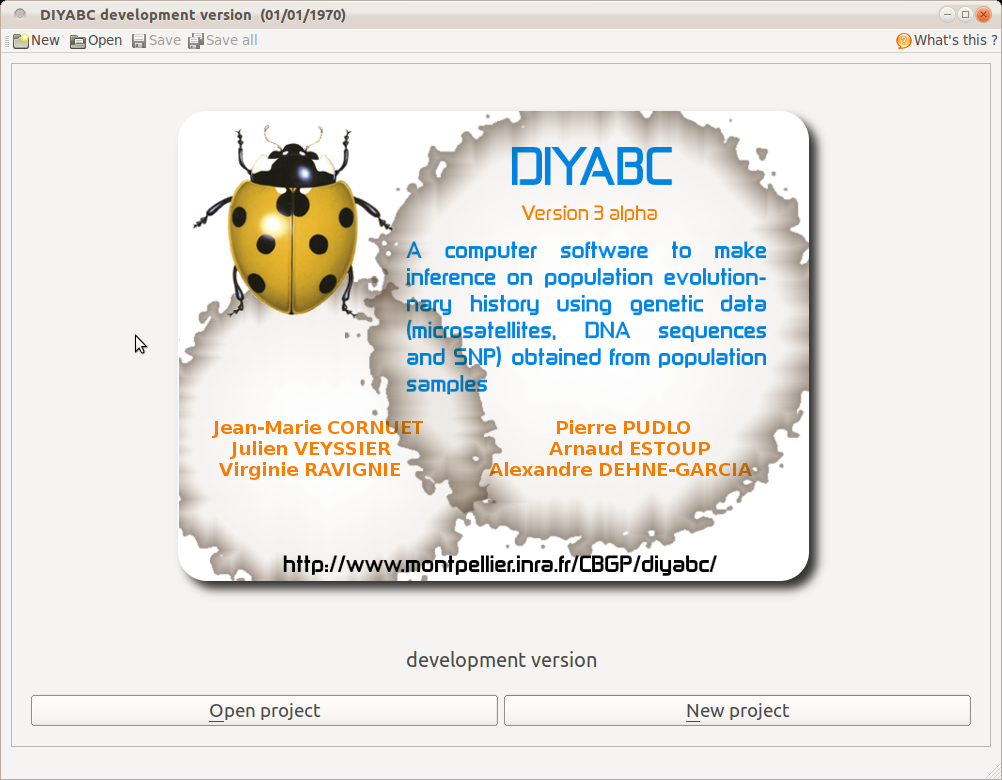
\includegraphics[scale=0.4]{gui_pictures/Capture-DIYABC-1.png} 

You can already notice that $DIYABC$ works with projects. This notion is new to version 2 of $DIYABC$. It is explained in subsection 3.1.

\subsection{What is a $DIYABC$ Project ?}

\label{doc_openProjectButton}
A $DIYABC$ project is a unit of work materialized by a specific and unique directory. A project is defined by at least one observed data set and one reference table header file. These files are located in the \emph{Project directory} which name includes an identifier, the date of creation and a number (between 1 and 100).\\

The header file, always named \texttt{header.txt}, contains all information necessary to compute a reference table associated with the data : i.e. the scenarios, the scenario parameter priors, the characteristics of loci, the loci parameter priors and the summary statistics to compute.
As soon as the first records of the reference table have been saved in the reference table file,  always named \texttt{reftable.bin} and also included in the project directory, the project is "locked". This means that the header file can not be changed anymore. If one needs to change a scenario or a parameter prior, or a summary statistics, a new project needs to be defined. This is to guarantee that all subsequent actions performed on the project are in coherence with the current data and header files. It is of course strongly advised NOT to move files among projects.
Incidentally, the \texttt{header.txt} file is only built when the project has been saved, the information progressively input by the user being saved in a series of temporary files.\\

Once a sufficiently large reference table has been simulated, analyses can be performed. Their different output files are copied to the \emph{analysis} directory included in the project directory, and containing as many directories as analyses performed. Hence, it is now much easier to know with certainty the conditions of each analysis.    

\subsection{Options of the home screen}
The home screen above has two menus and several buttons.\\ 
Let's start with the menus. Below are shown all submenus :

\begin{center} 
\begin{tabular}{cc}
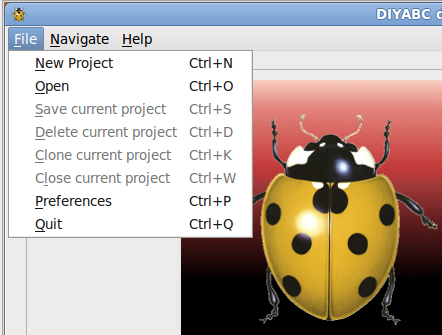
\includegraphics[scale=0.5]{gui_pictures/Capture-DIYABC-2.png} & 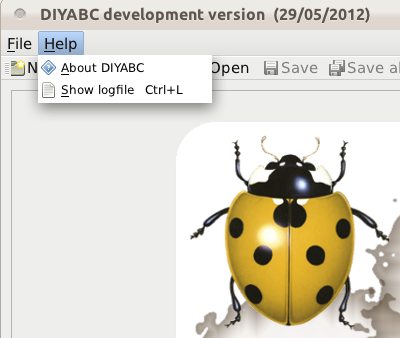
\includegraphics[scale=0.5]{gui_pictures/Capture-DIYABC-3.png}\\
\end{tabular}
\end{center}

The \texttt{File} menu has seven options, namely \texttt{New project}, \texttt{Open project}, \texttt{Open recent projects}, \texttt{Save all projects}, \texttt{Settings}, \texttt{Simulate data set(s)} and \texttt{Quit}. All are self explanatory.\\
The \texttt{Help} menu has two options : \texttt{About DIYABC} which opens up a small window providing the names and address of the authors and \texttt{Show logfile} which gives access to a logfile viewer in which are recorded all actions and messages about the execution of the GUI.\\ 
Just below the menu are five shortcuts to main \texttt{File} menu options.\\

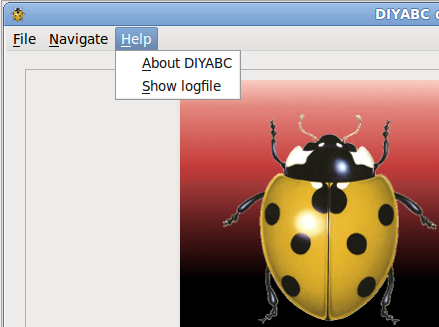
\includegraphics[scale=0.4]{gui_pictures/Capture-DIYABC-4.png}\\
 
On the right, the field \texttt{What's this ?} is an another way to get help on a specific GUI object :\\
 
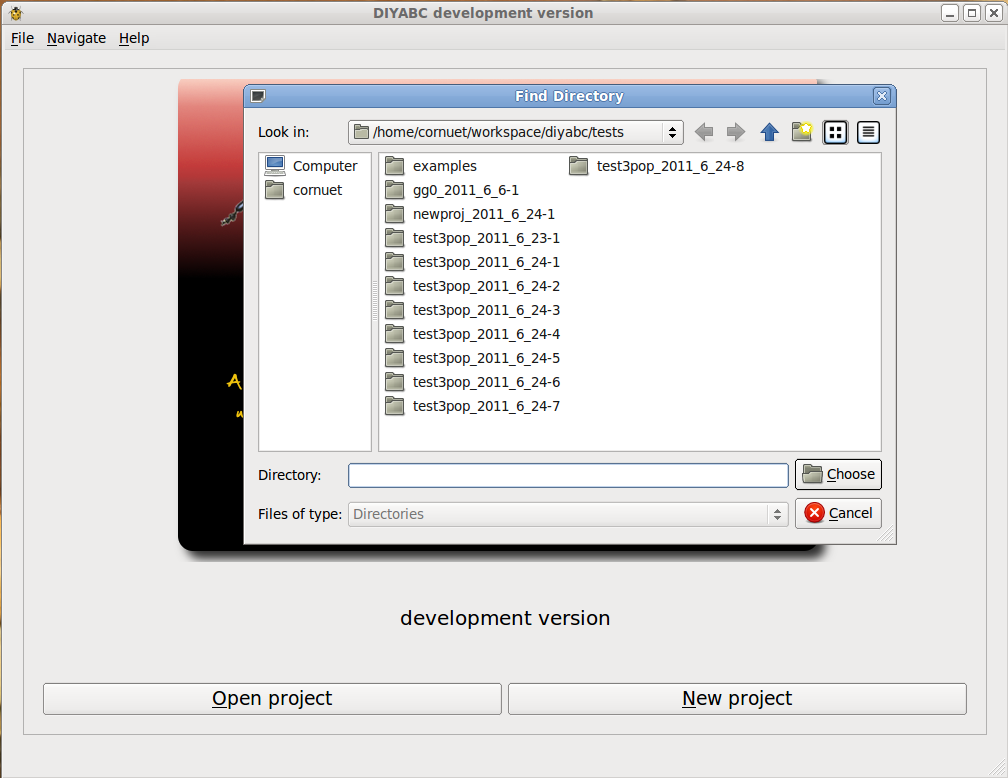
\includegraphics[scale=0.4]{gui_pictures/Capture-DIYABC-5.png}\\ 

Eventually, below the logo, there are three buttons which are duplicate shortcuts :\\
 
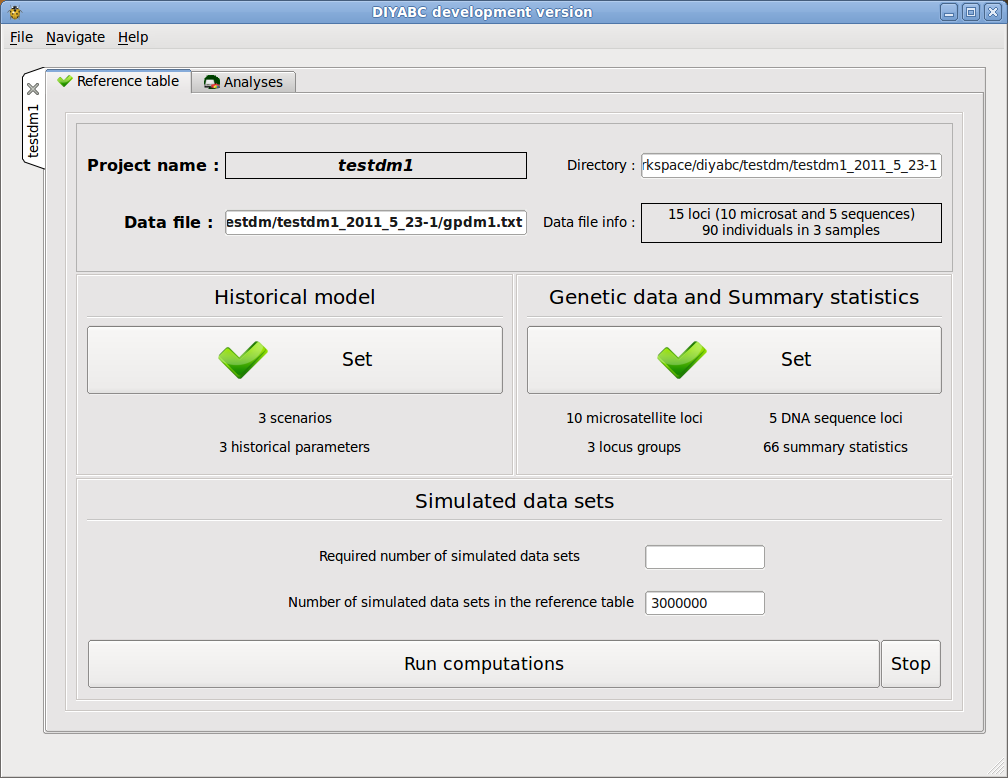
\includegraphics[scale=0.4]{gui_pictures/Capture-DIYABC-6.png}\\ 


The \texttt{Help} buttons has two options, the usual ``about'' giving information on the current version and the authors and a \texttt{Show logfile} which opens up a window showing the list of actions performed by the program.\\
  
Clicking on the \fbox{\textsf{Open project}} button opens up the following frame:\\

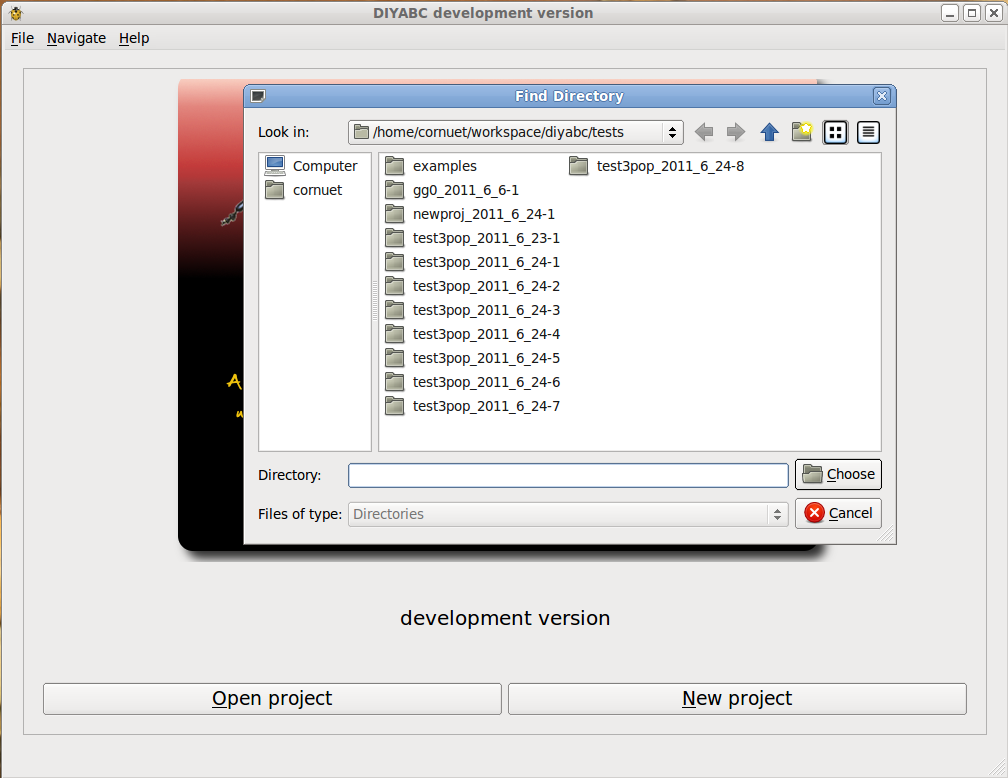
\includegraphics[scale=0.4]{gui_pictures/Capture-DIYABC-5.png} 

To select a project, you just double click on the corresponding directory.
\newpage
 The following screen then appears :\\

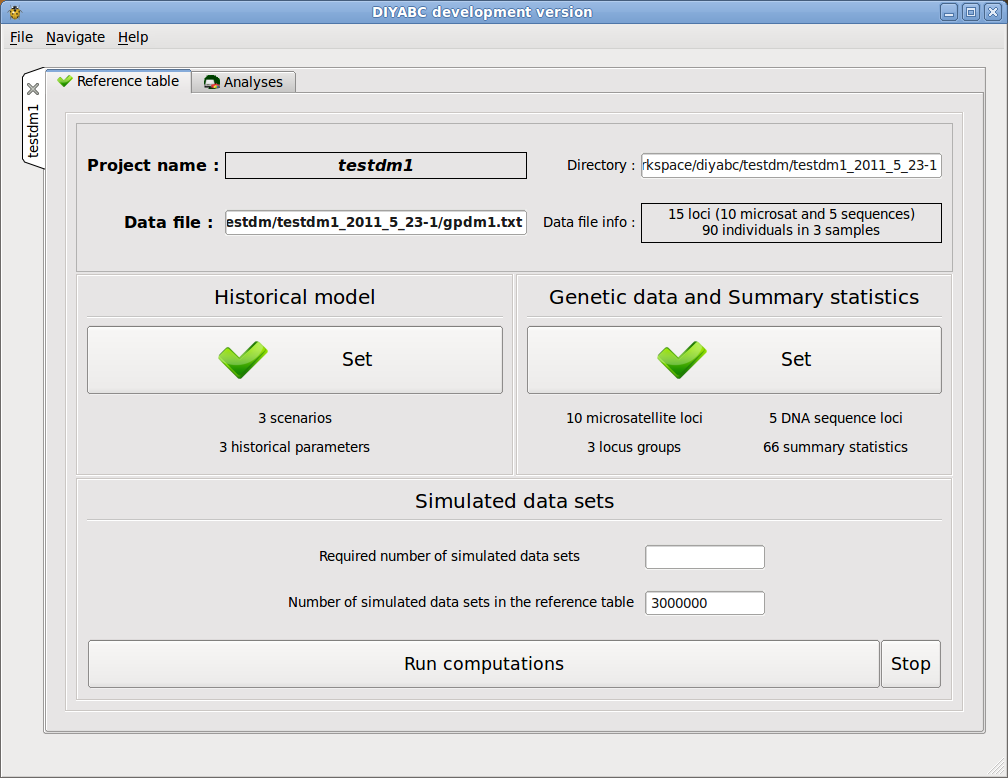
\includegraphics[scale=0.35]{gui_pictures/Capture-DIYABC-6.png} 

We will go back later to the description of this screen.
\begin{itemize}
 \item 
  Cliking on the \fbox{\textsf{New project}} opens up the screen below requiring a name for the new project :\\
\begin{center}
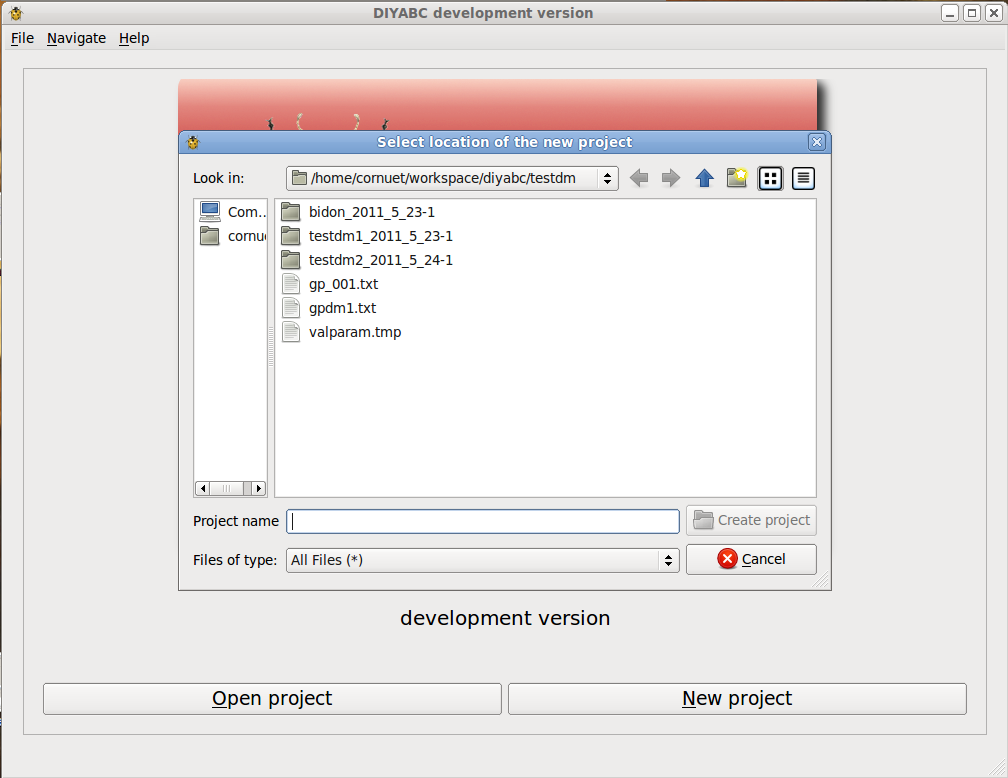
\includegraphics[scale=0.35]{gui_pictures/Capture-DIYABC-7.png} 
\end{center}
\item
After giving a name to new project and cliking on \fbox{\textsf{OK}}, the following screen appears :\\ 

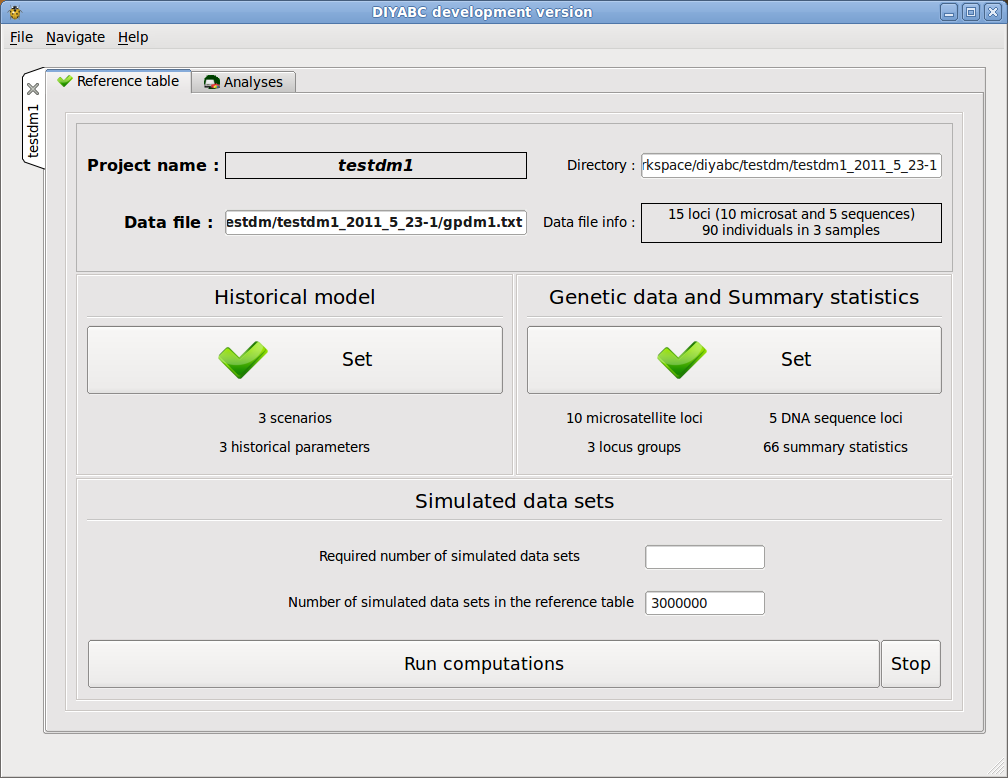
\includegraphics[scale=0.35]{gui_pictures/Capture-DIYABC-6.png} 

\end{itemize}

\subsection{Defining a new project}
Defining a new project requires to follow a number of steps that we are going to detail now.

\subsubsection{Step 1 : choosing the data file}
This is performed by clicking on the corresponding \fbox{\textsf{Browse}} button (previous screen).  The usual file browsing screen appears (below) and one has to select a Genepop format data file, here \texttt{gg\_001.txt}. \\

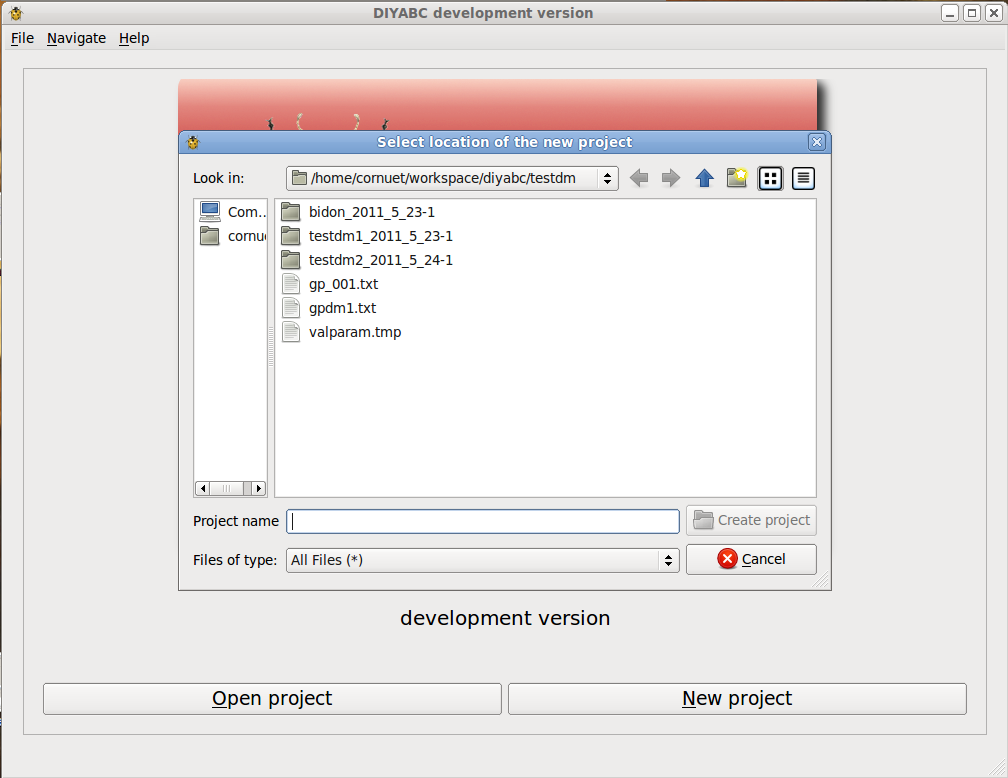
\includegraphics[scale=0.35]{gui_pictures/Capture-DIYABC-7.png} 

Clicking on the \fbox{\textsf{Open}} button leads back to the previous screen with the edit field filled with the name of the data file and some characteristics of this data file appearing on the screen (number of loci, individuals and samples).\\

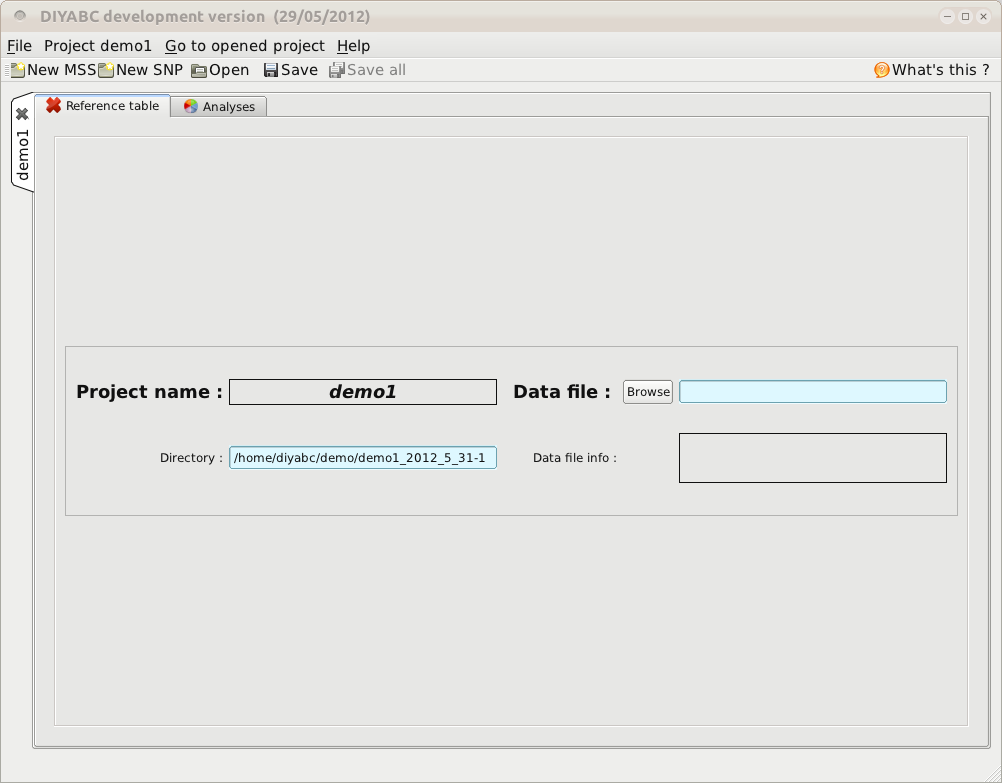
\includegraphics[scale=0.35]{gui_pictures/Capture-DIYABC-8.png} 

\subsubsection{Step 2 : choosing the location of the project directory}
 Click on the corresponding \fbox{\textsf{Browse}} button (previous screen). The usual directory browsing screen appears (below). 
 
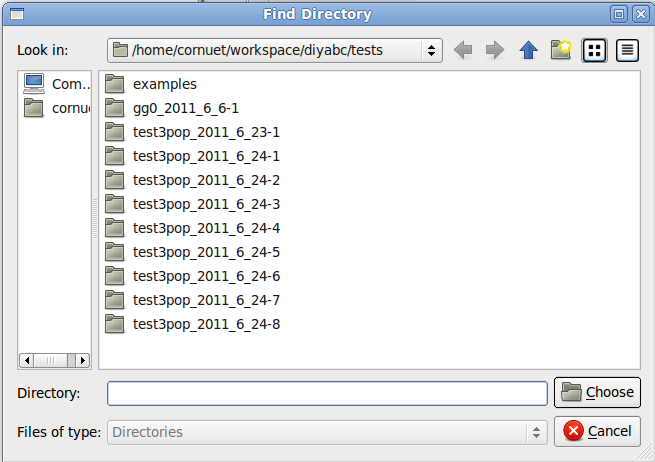
\includegraphics[scale=0.35]{gui_pictures/Capture-DIYABC-9.png} 
 
Clicking on the  \fbox{\textsf{Choose}} button will create the new project directory in the \texttt{/home/cornuet/workspace/diyabc/tests} directory as shown in the screen below.\\  

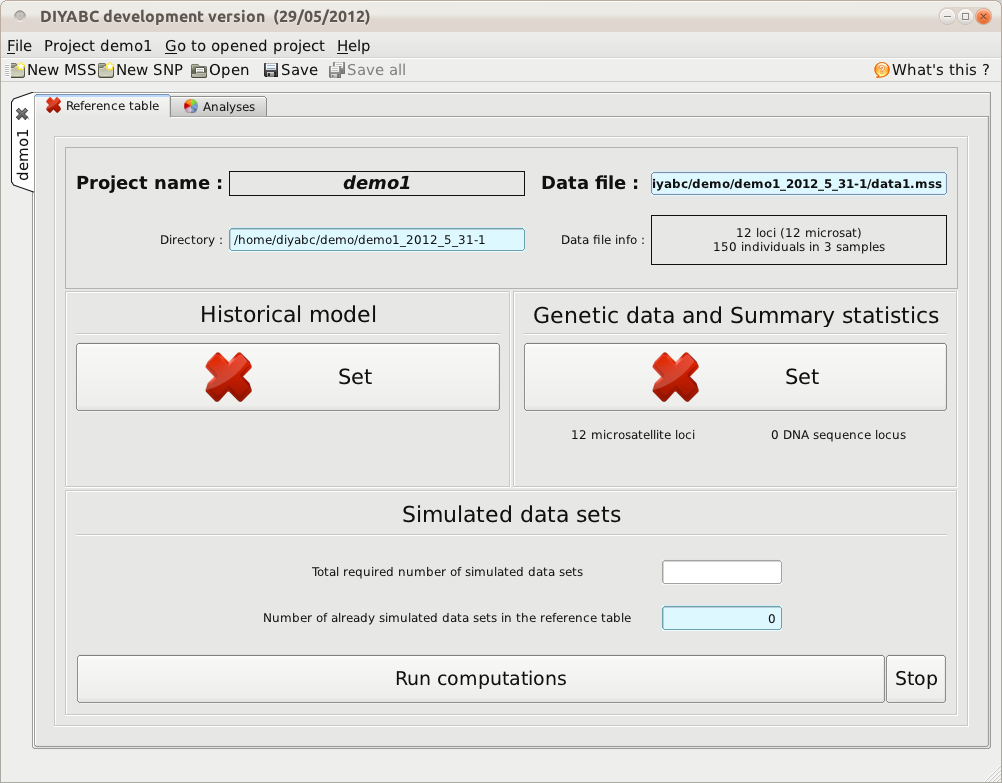
\includegraphics[scale=0.35]{gui_pictures/Capture-DIYABC-10.png} 
 \vfill
 Three new frames have appeared on the screen : Historical model, Genetic data/Summary statistics and Simulated data sets. The first two screens show a red cross meaning that they require information from the user. Once this information will be input and validated, the red cross will change to a green check sign as already shown on page 18.
 
 \newpage
\subsubsection{Inform the Historical model}
Click on the corresponding \fbox{\textsf{Set}} button. The following screen, familiar to users of previous versions, appears:\\

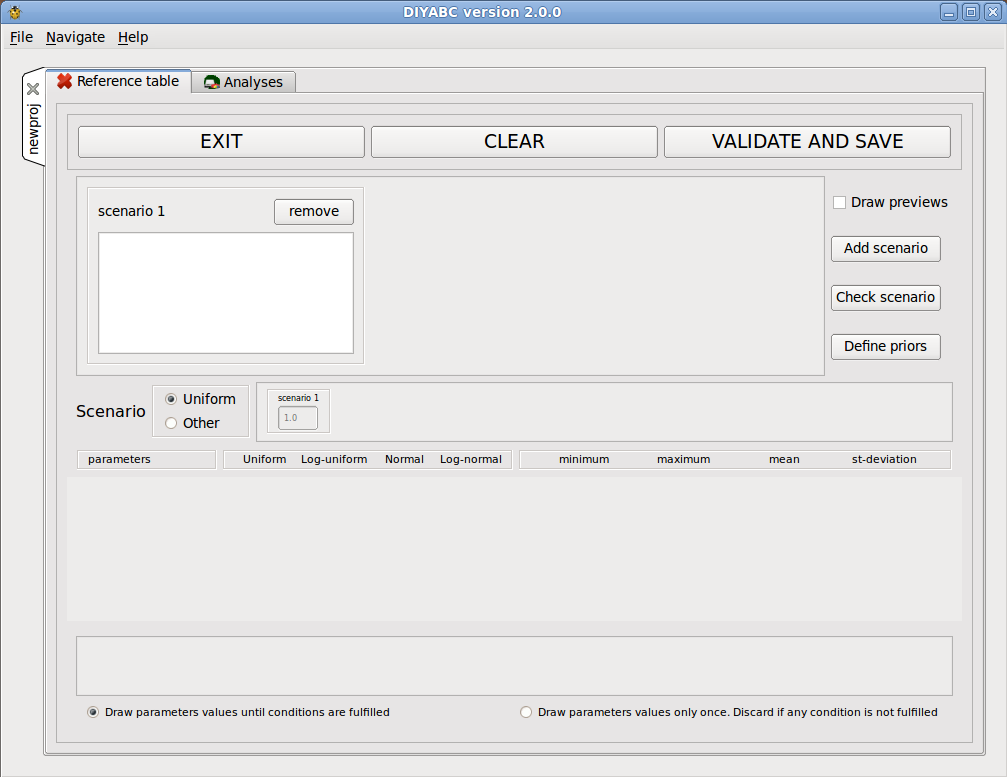
\includegraphics[scale=0.35]{gui_pictures/Capture-DIYABC-11.png} 

Let's enter a simple scenario in scenario 1 edit window and click on the \fbox{\textsf{Define priors}} button. We get this :\\

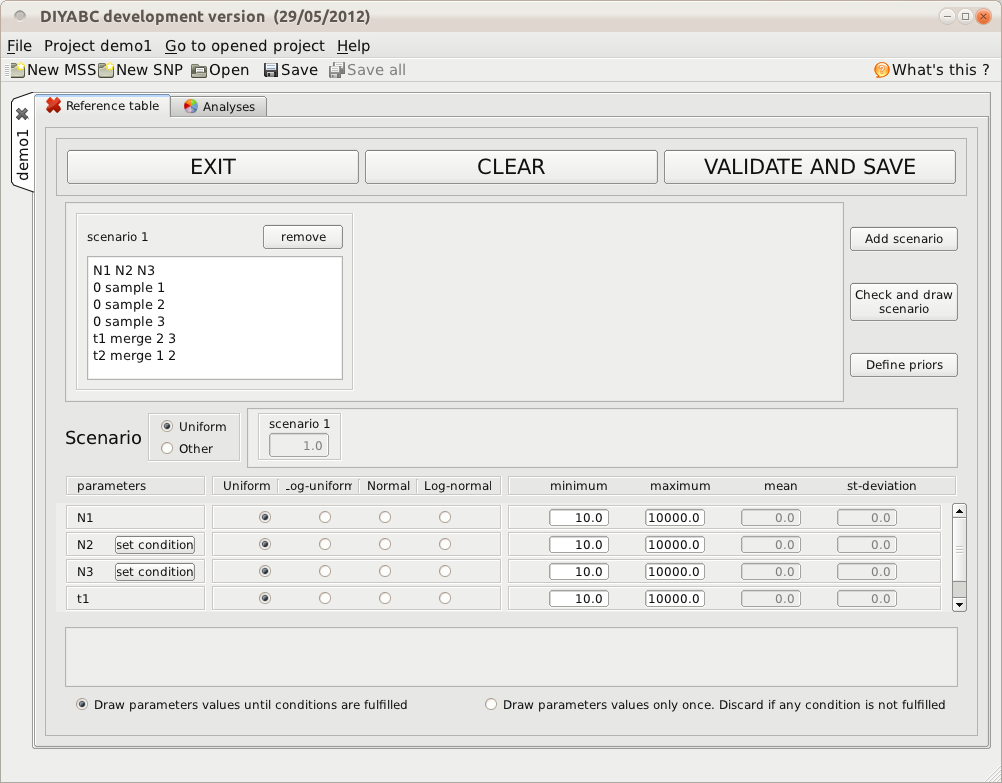
\includegraphics[scale=0.35]{gui_pictures/Capture-DIYABC-12.png} 

The parameter prior frame allows to choose the prior density of each parameter. A parameter is anything in the scenario that is not a keyword (here \texttt{sample,split} and \texttt{merge}), nor a numeric value. In our little scenario, parameters are hence : \texttt{N1, N2, N3, t1, r1} and \texttt{t2}.\\

If we click on the \fbox{\textsf{Check scenario}} button, the logic of the scenario is checked and if it is found OK, and if the scenario is drawable, the drawing appears on a new frame : \\

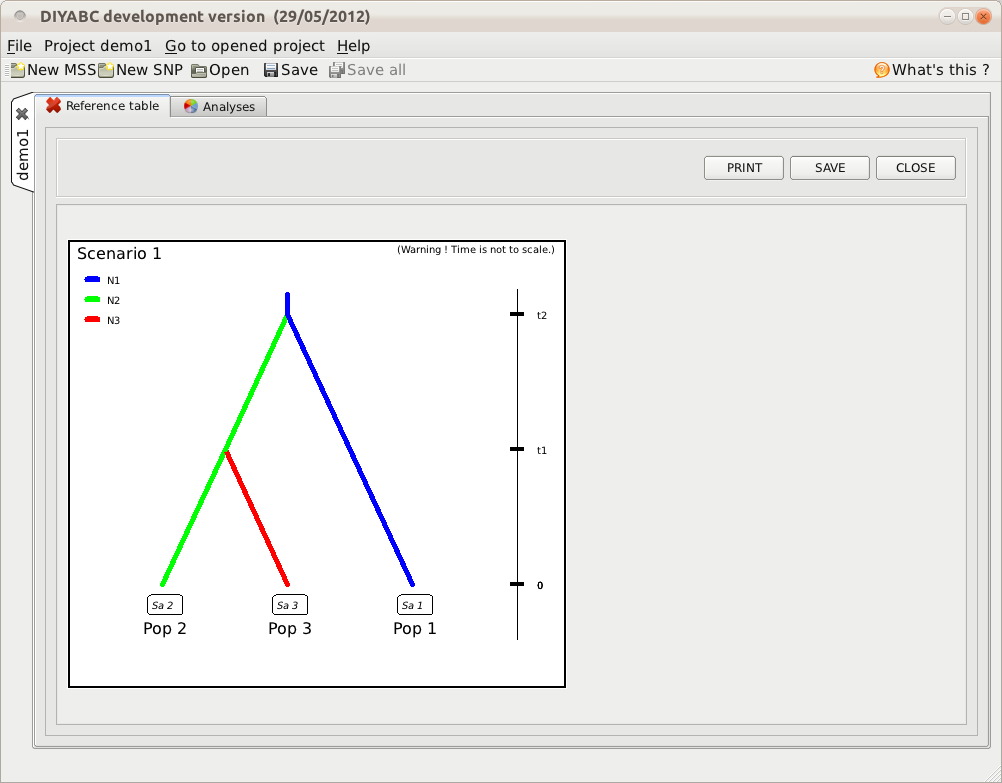
\includegraphics[scale=0.35]{gui_pictures/Capture-DIYABC-13.png} 

The scenario can be saved by clicking on the \fbox{\textsf{SAVE}} button. The frame can be close by clicking on the \fbox{\textsf{CLOSE}} button.\\

Since the scenario has been checked, we can validate and save the historical model by clicking on the  \fbox{\textsf{VALIDATE AND SAVE}} button (bottom screen of p 21). We go then go back to the project screen in which the historical model has now received the green check sign.\\

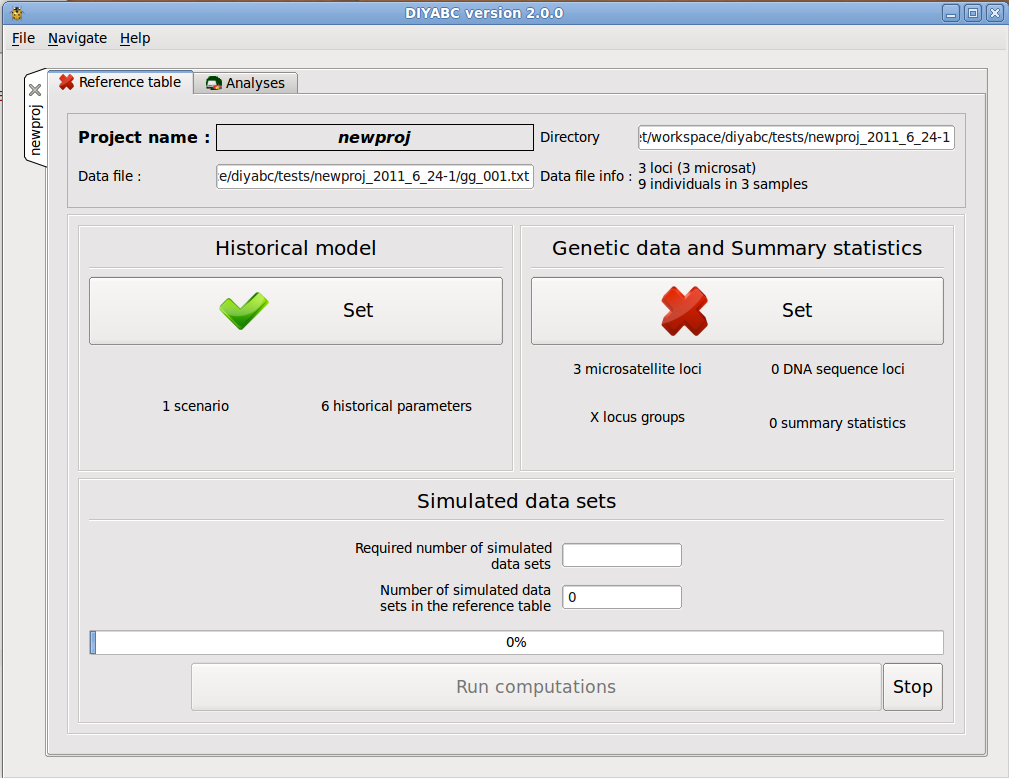
\includegraphics[scale=0.35]{gui_pictures/Capture-DIYABC-14.png} 

 \newpage
\subsubsection{Inform the Genetic model}

Click on the corresponding \fbox{\textsf{Set}} button. We get the following screen : \\

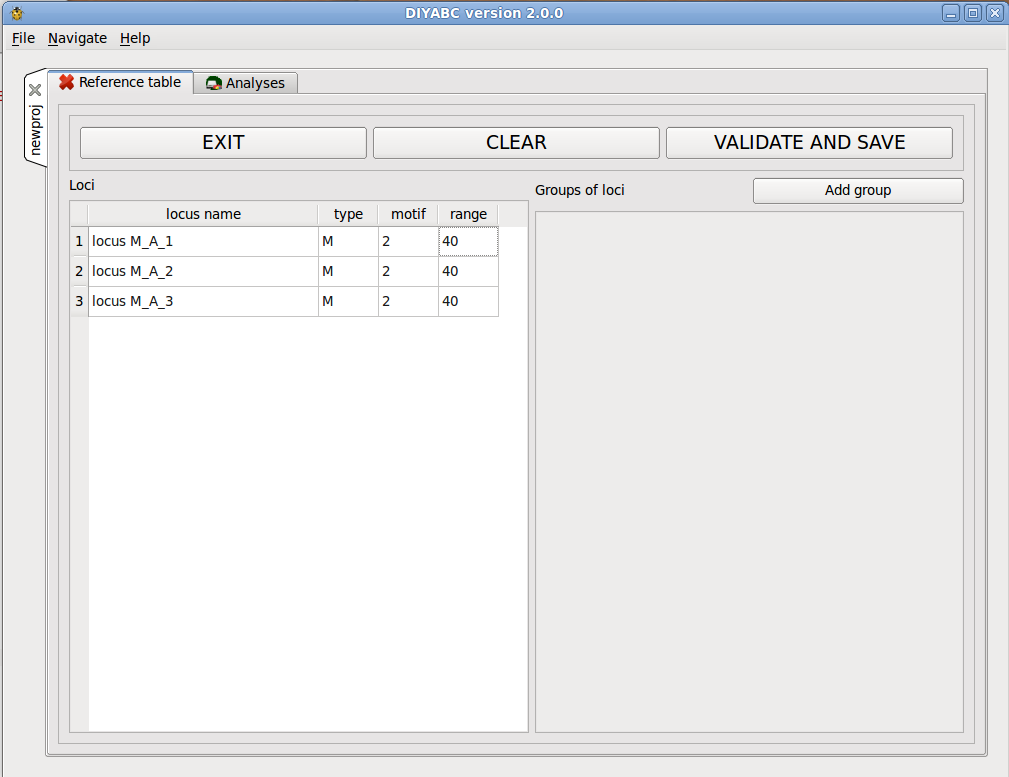
\includegraphics[scale=0.35]{gui_pictures/Capture-DIYABC-15.png} 

On the left part of the screen, there is the list of loci, with their type (M for microsatellites or S for DNA sequences) and the motif size and range for microsatellite loci only. Actually, the values for motif size and range are just default values and do not necessarily correspond to the actual data. The user who knows the real values for its data is required to set the correct values at this stage. If the range is to short to include all observed values, a message appears in a box asking to enlarge the corresponding range. Note that the range is measured in number of motifs, so that a range of 40 for a motif length of 2 bp means that the difference between the smallest and the longest alleles should not exceed 80 bp.\\
We then need to define at least one group of loci by clicking on the \fbox{\textsf{Add group}} button. We get this :\\

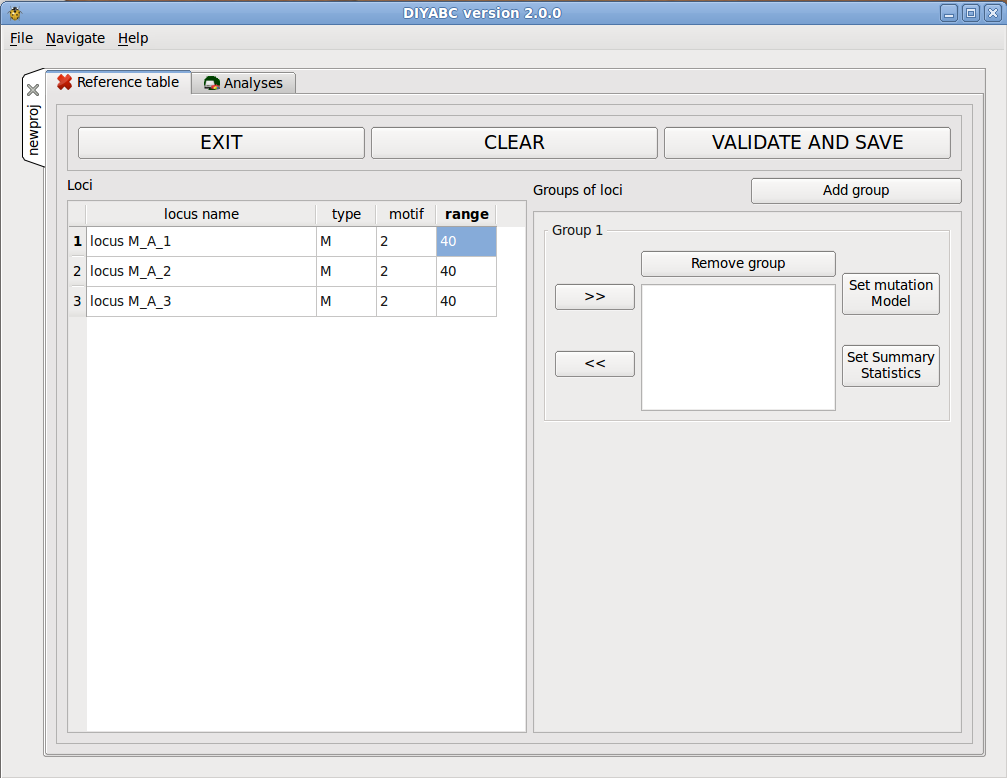
\includegraphics[scale=0.35]{gui_pictures/Capture-DIYABC-16.png} 

Suppose we want the three loci in the same group. We select them like in any table, extending the selection with the \texttt{Shift} and \texttt{Control} keys (see below) : \\

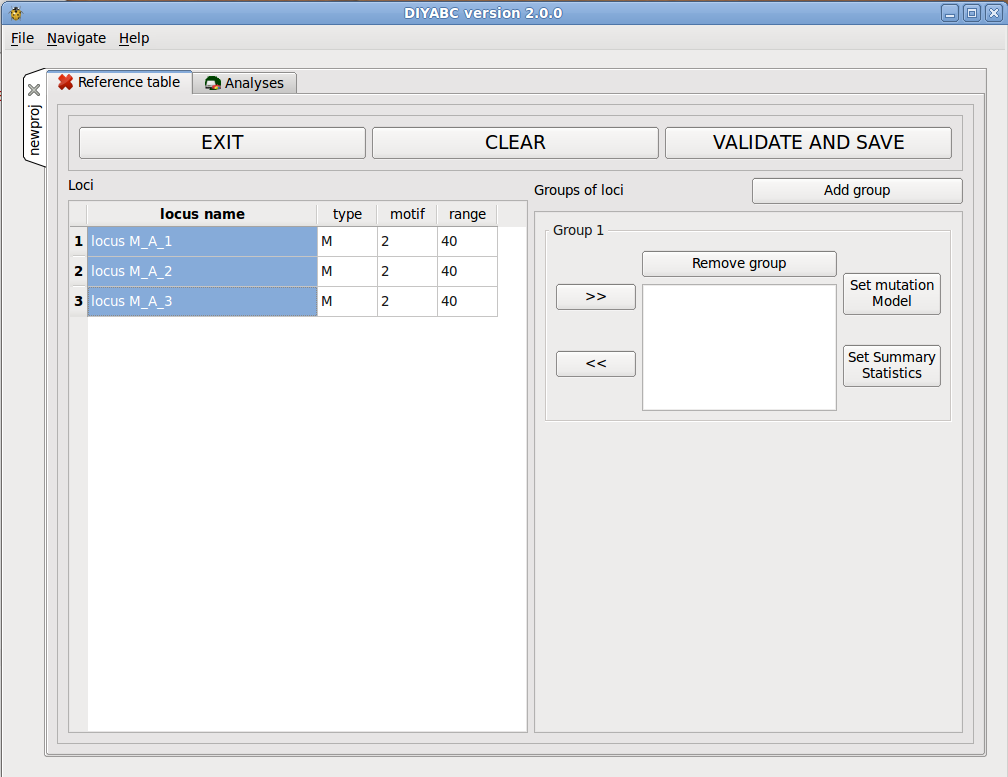
\includegraphics[scale=0.35]{gui_pictures/Capture-DIYABC-17.png} 

and then pressing the \fbox{\textsf{$ >> $}} button : \\

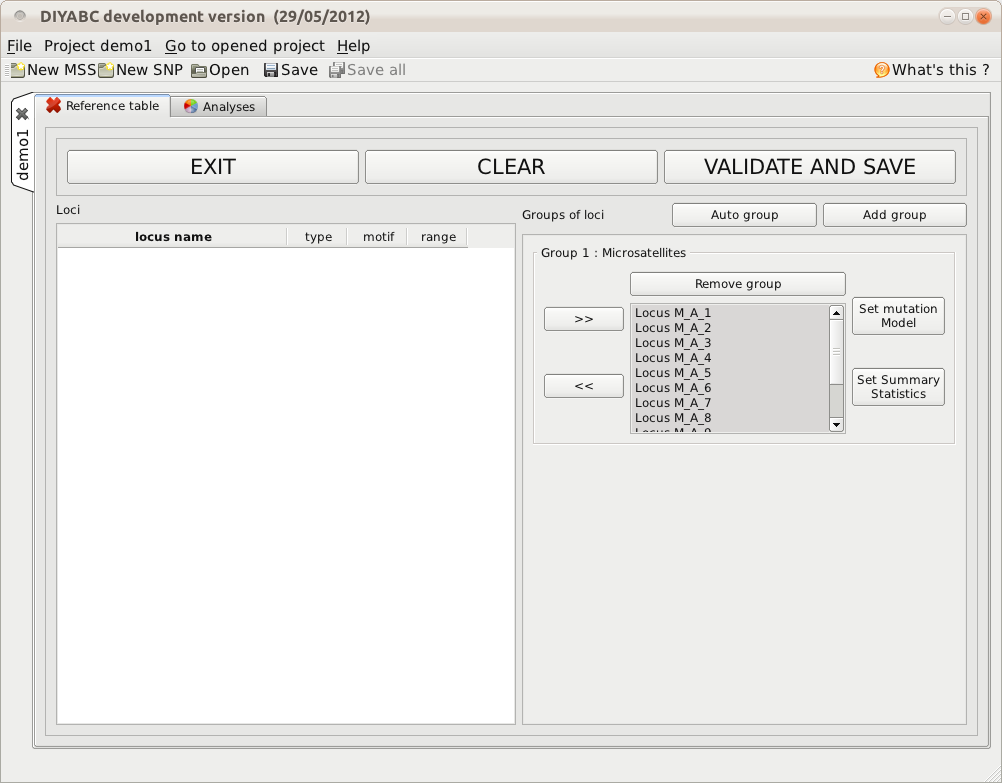
\includegraphics[scale=0.35]{gui_pictures/Capture-DIYABC-18.png} 

We then need to define the mutation model and the summary statistics of the locus group. Clicking on the \fbox{\textsf{Set mutation model}} button, the following screen appears :\\

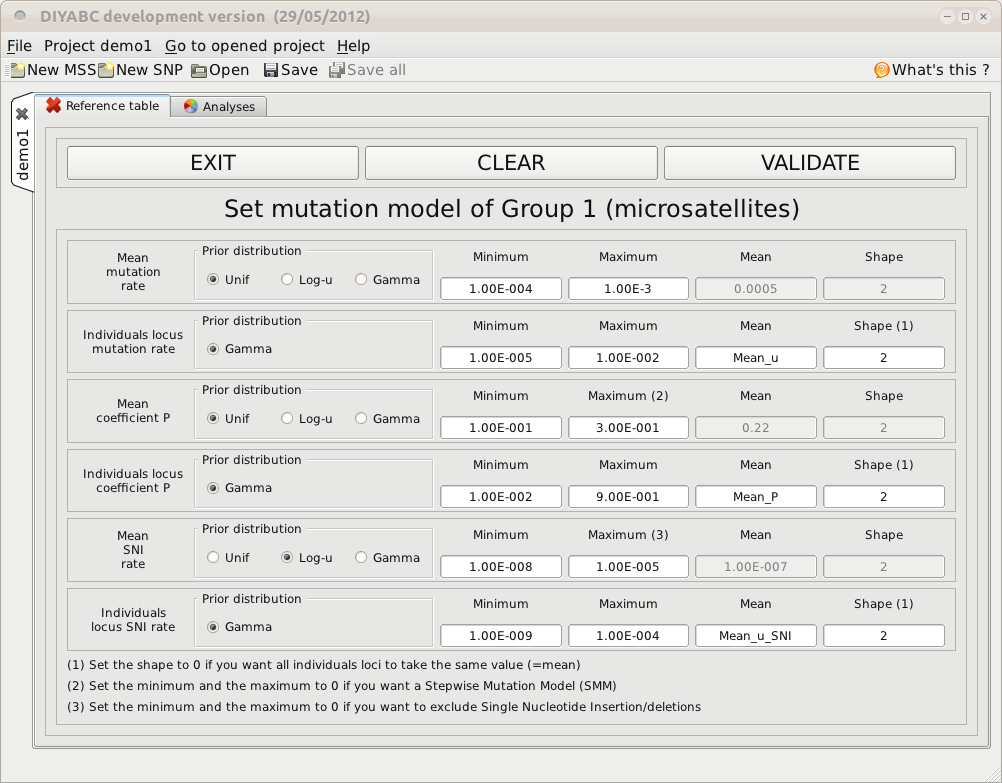
\includegraphics[scale=0.35]{gui_pictures/Capture-DIYABC-19.png} 

Once the mutation model of Group 1 is defined, we click on the \fbox{\textsf{VALIDATE}} button to go back to the previous screen.

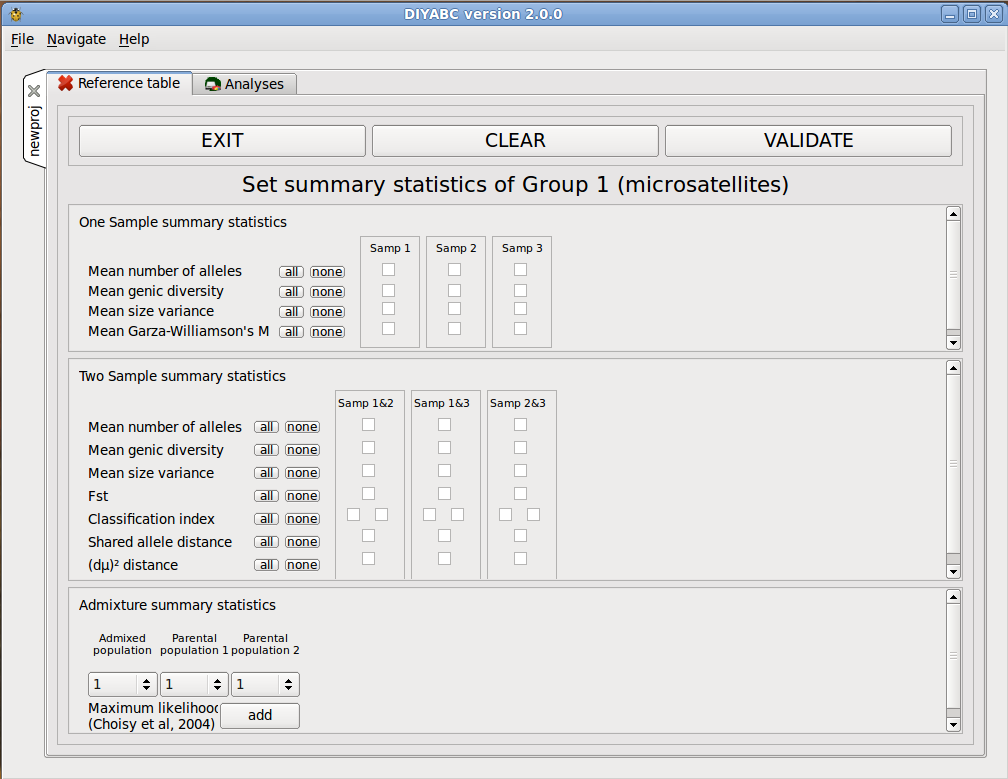
\includegraphics[scale=0.35]{gui_pictures/Capture-DIYABC-20.png} 

We define summary statistics by checking the corresponding boxes :\\ 

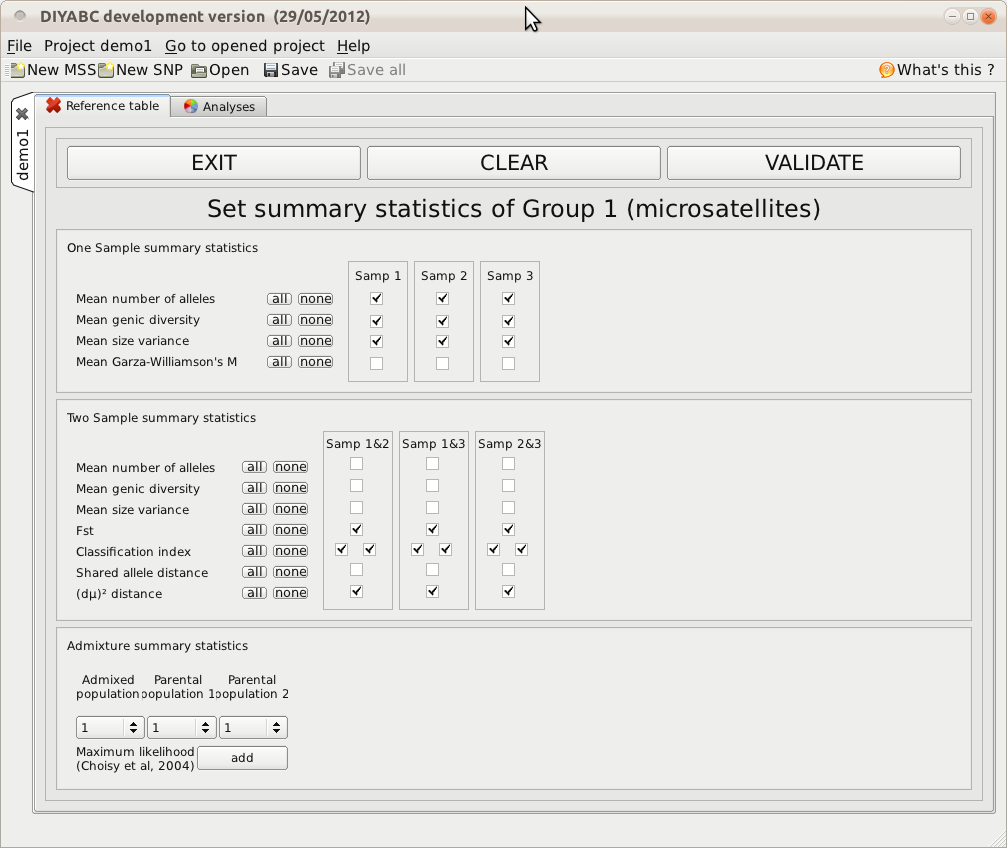
\includegraphics[scale=0.35]{gui_pictures/Capture-DIYABC-21.png} 

Once finished, we click on the \fbox{\textsf{VALIDATE}} button to go back to the screen of p24. Now, we can validate also this screen which brings us back to the screen of p22. The latter looks now like this : \\

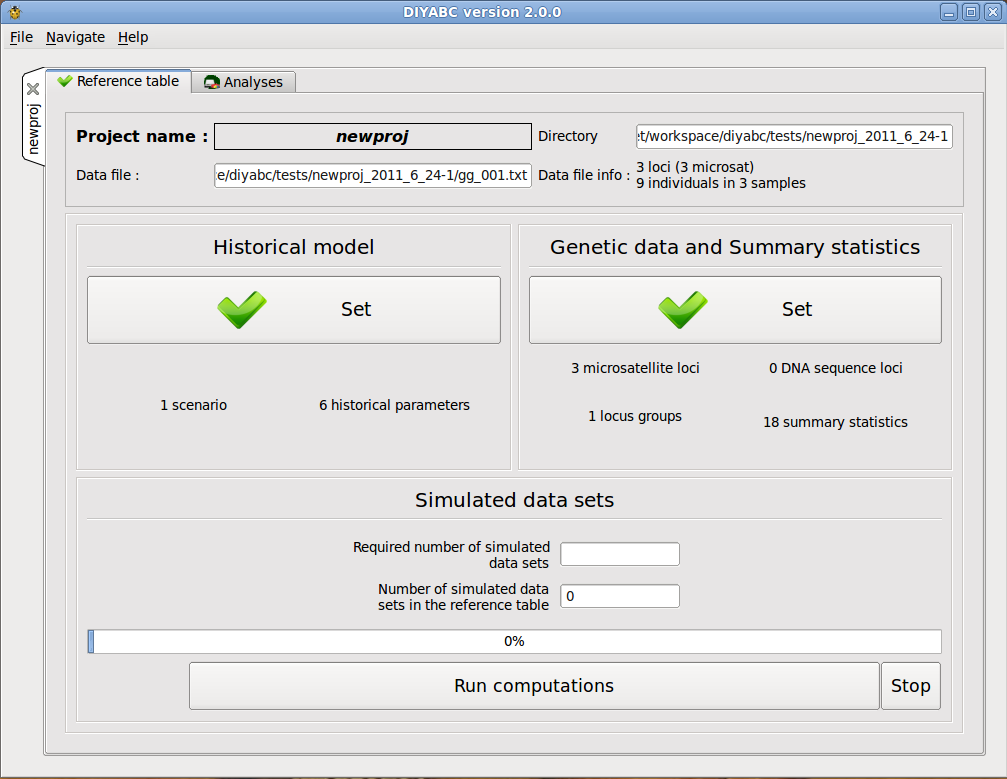
\includegraphics[scale=0.35]{gui_pictures/Capture-DIYABC-22.png} 

At that moment, the project directory includes the following files : a copy of the data file, and four configuration files : \texttt{conf.analysis}, \texttt{conf.gen.tmp}, \texttt{conf.hist.tmp}, \texttt{conf.tmp}. Note that the project is not yet saved. To save the project, we need either to save it explicitly by using the \texttt{File} menu (see below) or to start simulating data sets (next section). Saving the project results in saving the \texttt{header.txt} file in the project directory.


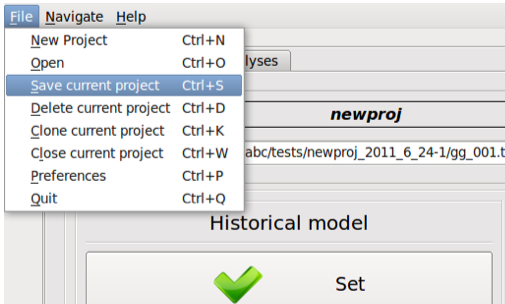
\includegraphics[scale=0.35]{gui_pictures/Capture-DIYABC-23.png} 

\subsection{Building the reference table}

Keeping on the current screen, indicate the required number of data sets to simulate for the reference table : \\ 

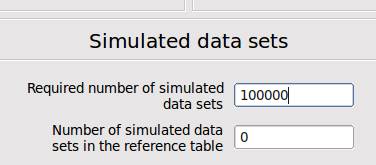
\includegraphics[scale=0.35]{gui_pictures/Capture-DIYABC-24.png} 


Then click on the \fbox{\textsf{Run computations}} button. If things go well, you will soon see the progress both into the edit window "Number of simulated data sets in the reference table" and in the progress bar below. Also, you have an estimate of the remaining time (at the left of the  \fbox{\textsf{Run computations}} button):\\

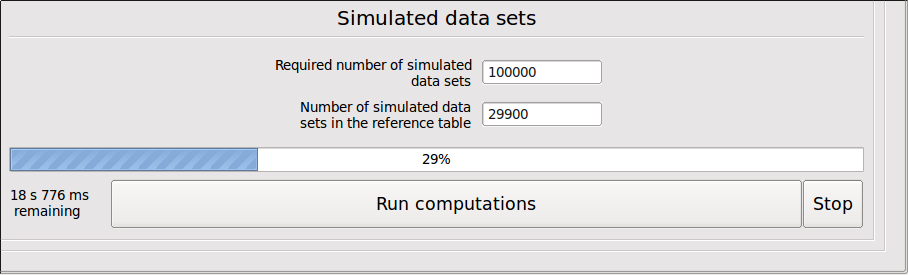
\includegraphics[scale=0.35]{gui_pictures/Capture-DIYABC-25.png} 

When the computation is finished, the screen looks like this :\\

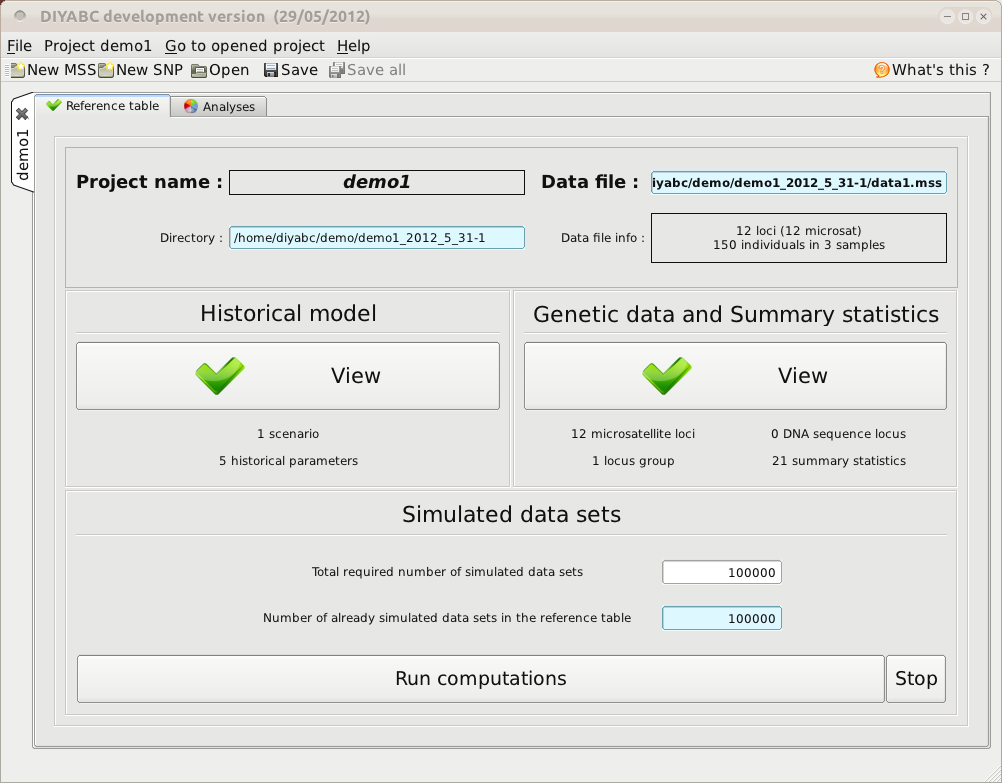
\includegraphics[scale=0.35]{gui_pictures/Capture-DIYABC-26.png} 



\clearpage
 \section{Implementation details}
\subsection{Software design}
$DIYABC$ v2 has been designed in a very different way compared to version 1. Version 1 was a single executable file were the GUI \footnote{Graphic User Interface} and computation codes were highly intricated and both written in the same language (\emph{Delphi}). In version 2, the GUI and the computation codes have been completely separated. Actually, the GUI is a script written in \emph{python} and all computations are included in a program written in \emph{C++}. In opposition to \emph{Delphi} which is restricted to a single OS (\texttt{Windows}), \textit{python} and \textit{C++} can be used with the main three OS (\texttt{Linux}, \texttt{Mac} and \texttt{Windows}), allowing version 2  to be operated under all three OS.\\
The GUI uses the \textit{Qt} graphic library. The computation code is linked to the \textit{openmp} library allowing a better use of multicore/multiprocessor computers.\\
The GUI can launch the computation program with the right parameters and keeps track of the progress of the latter through small log files. The GUI can launch as many computation programs as there are open projects, but no more than one computation program per project. A \textit{lock} file located in the project directory is created when the computation program is launched by the GUI and removed when the computation program has normally terminated. When the computation program has exited anormaly, the GUI issues an error message trying to explain where the programm failed.    
\subsection{Files}
The program uses and produces various files which we will describe now.
\subsubsection{data files}
Data files are text files that contain information about the samples : number and names of microsatellite markers, multilocus genotypes of individuals. The basic  format is that of the Genepop software \citep{RR1995} and data files produced by DIYABC are under this format.  \textbf{Microsatellite genotypes must be noted with 3 (haploid) or 6 (diploid) digits, these three digit numbers being the length in nucleotides of the corresponding PCR products}. In addition, we have added some features to this basic format in order to use sequence data. All these additions are explained in section 4.4. SNP data correspond to a different file format, also detailed in section 4.4.\\ 
Any extension is accepted for datafile names, including no extension at all. If the data file is simulated with $DIYABC$, the extension is \texttt{mss} for microsatellite/DNA sequence data and \texttt{snp} for SNP data. The next page shows examples of data sets saved.

\subsubsection{reference table files} 
Reference table files are binary files which include two successive parts :
\begin{itemize}
 \item The first part is a header which contains information necessary to read the second part, such as the number of scenarios, or the number of parameters of each scenario.
 \item The second part contains simulated data set records, each record containing the scenario number, the parameter and summary statistics values.
\end{itemize}
 
 Each time a reference table is created or increased (each time the \fbox{\textsf{Run computation}} button is pressed), a text file is created in the project directory with the name \texttt{first\_records\_of\_the\_reference\_table\_X.txt} in which \texttt{X} is an integer number starting at 0 and increasing each time the \fbox{\textsf{Run computation}} button is pressed. This file provides a text version of the first $n$ newly created records of the reference table ($n$ being equal to the \emph{Particle loop size}, see section 3.7.3).\\

\subsubsection{output files}
As already seen, DIYABC achieves different analyses : comparison of scenarios, estimation of posterior distribution of parameters, model checking,  computation of bias and mean square errors and evaluation of confidence in scenario choice. Each analysis has its own output which can be printed and saved. Graphs are saved under the chosen format and non-graphic output are saved in text files.\\

We now describe all the files produced by each type of analysis. These files are located in directories (one directory per analysis) gathered in the \texttt{analysis} subdirectory of the project directory. Below is an example of the \texttt{TOYTEST2\_2012\_9\_26-1} project directory substructure:\\

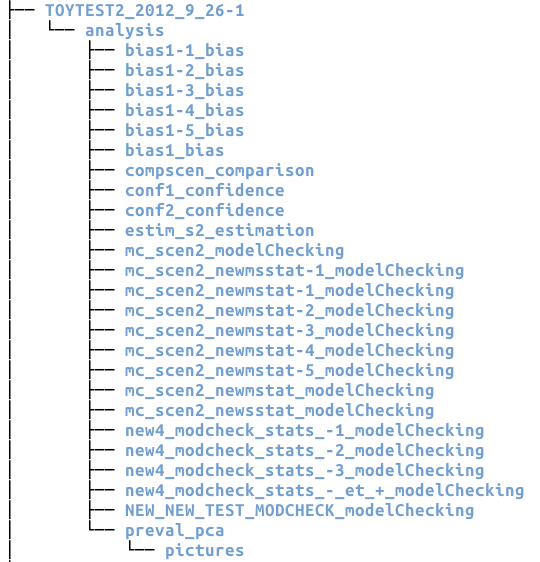
\includegraphics[scale=0.5]{gui_pictures/Capture-DIYABC-103.png}\\

Note that each directory name starts with the name of analysis followed by the type of analysis, $e.g.$ \texttt{bias} for a bias/precision analysis or \texttt{comparison} for a comparison of scenarios. In addition, when a picture has been saved, the corresponding file is located under a subdirectory named \texttt{pictures} ($e.g.$ at the bottom of the figure above).
\begin{description}
 \item [Pre-evaluate scenario prior combinations :] This analysis can produce two output files named \texttt{ACP.txt} and \texttt{locate.txt}. The former is the output of the Principal Component Analysis and the latter that of the analysis giving the proportion of simulated data sets which have a value below the observed value for every summary statistics. This latter file is exactly what appears in the GUI. The structure of the  \texttt{ACP.txt} file is the following. The first line indicates the number of points of the PCA, the number of PCA components (axes) and the inertia of each component, all values are separated by a single space. The second line provides the components of the observed data. It starts with a zero which corresponds to the scenario number in the following lines. Each subsequent line provides the components of data simulated according to a given scenario which number is at the beginning of the line. If one or more PCA figures have been saved, the corresponding files are saved in the \texttt{pictures} subdirectory. They are named as \texttt{refTable\_PCA\_X\_Y\_N.pdf}, with \texttt{X} and  \texttt{Y} giving the axis numbers and \texttt{N} being the number of represented points. 
 \item [Compute posterior probabilities of scenarios :] This analysis produces three output text files : \texttt{compdirect.txt}, \texttt{complogreg.txt} and \texttt{compdirlog.txt}. The latter is directly visualized in the GUI when clicking the \fbox{\textsf{view numerical results}} button. The first two files are used by the GUI to elaborate the two graphics (Direct approach and Logistic regression). Again, if graphics have been saved, the corresponding file(s) is(are) in the \texttt{pictures} subdirectory of the analysis directory.  
 \item [Evaluate confidence in scenario choice :] This analysis produces a single output file, \texttt{confidence.txt}, the content of which is visualized in the GUI.
 \item [Estimate posterior distributions of parameter :] Nine files are written as output of this type of analysis :
  \begin{itemize}
   \item three files \texttt{mmmq\_original.txt}, \texttt{mmmq\_composite.txt} and \texttt{mmmq\_scaled.txt} contain the statistics (mean, median, mode and quantiles) for the original, composite and scaled parameters, respectively. They are visualized in the GUI when clicking the \fbox{\textsf{view numerical results}} button. 
   \item three files \texttt{paramstatdens\_original.txt}, \texttt{paramstatdens\_composite.txt} and \texttt{paramstatdens\_scaled.txt} are used by the GUI to produce the graphics showing prior/posterior distribution.
   \item three files \texttt{phistar\_original.txt}, \texttt{phistar\_composite.txt} and \texttt{phistar\_scaled.txt} contains the $\phi^*$ values of the original, composite and scaled parameters, respectively. These files can be used for instance to redraw posterior distributions, $e.g.$ with the $R$ software.
  \end{itemize}
As already mentionned, saved graphics are located in a \texttt{pictures} subdirectory.
 \item [Compute bias and precision of parameter estimations :] Three files \texttt{bias\_original.txt}, \texttt{bias\_composite.txt} and \texttt{bias\_scaled.txt} are produced by this type of analysis. All three files are visualized in the GUI. 
 \item [Perform model-checking] The output files of this type of analysis are the same as those of the \textit{Pre-evaluate scenario prior combinations} analysis (see above). The only difference is in the names of the two text files which start with \texttt{mc} for \texttt{model checking}. 
\end{description}
~\\

In addition, the GUI program writes several files in the project directory :
\begin{description}
 \item [command.txt :] this text file contains the history of commands issued by the GUI to be achieved by the computation program.
 \item [conf.analysis :] this text file contains information about analyses.
 \item [conf.gen.tmp :] this text file contains information about the loci, the genetic parameters and the summary statistics.
 \item [conf.hist.tmp :] this text file contains information about the scenario and the historical parameters.
 \item [conf.th.tmp :] This text file contains the title line of the reference table.
 \item [conf.tmp :] This text file contains the name of the dataset and the number of parameters and summary statistics.
 \item [header.txt :] This text file is a concatenation of the previous four files and is red by the computation program.
 \item [xxx.diyabcproject :] This text file contains the path to the \texttt{xxx} project.
 \item [RNG\_state\_0000.bin :] This binary file contains the current state of the random generator.
 \item [init\_rng.out :] This text file contains information about the initialization of the random generator.
\end{description}
~\\

The computation program writes the following files in the project directory :
\begin{description}
 \item [reftable.log :] This text file is produced when a reftable is increased. It provides the GUI with information about the progress of computations : achieved number of records, time left.
 \item [statobs.txt :] This text file is written every time an analysis is performed. It contains the values of summary statistrics for the observed data set.
\end{description}

The following files are output by the computation program everytime it has been launched by a specific command of the GUI (their use is only for debugging purposes and they are all in the project directory) :
\begin{description}
 \item [general.out :] when computing a reftable.
 \item [pre-ev.out :] when performing a \textit{Pre-evaluate scenario prior combinations} analysis.
 \item [compare.out :] when performing a \textit{Compare scenarios} analysis.
 \item [confidence.out :] when performing a \textit{Confidence in scenario choice} analysis.
 \item [estimate.out :] when performing a \textit{ABC parameter estimation} analysis.
 \item [bias.out :] when performing a \textit{bias-precision} analysis.
 \item [modelChecking.out :] when performing a \textit{model checking} analysis.
\end{description}

When performing a \textit{Bias-precision} or a \textit{Confidence in scenario choice} analysis, the computation program simulates what we call \textit{pseudo-observed datasets}. The parameter and summary statistics values of these pseudo-observed datasets are written in a text file named \textbf{pseudo-observed\_datasets\_xxx.txt} in which \textbf{xxx} is the name given to the analysis.


\subsection{Missing data}
Missing or undetermined genotypes should be coded as \texttt{000} (haploid microsatellites), \texttt{000000}  (diploid microsatellites), \texttt{$<[~]>$} (haploid sequences) or \texttt{$<[~][~]>$} (diploid sequences) and \texttt{9} (SNP) in the data file. \\
Missing data are taken into account in the following way. For each appearance of a missing genotype in the observed data set, the programs records the individual and the locus. When simulating data sets, the program replaces the simulated genotype (obtained through the coalescence process algorithm) by the missing data code at all corresponding locations. All summary statistics are thus computed with the same missing data as for the observed data set. 

\subsection{Data files}
There are two different incompatible formats for data files, one for SNP loci and the other for microsatellite/DNA sequence data.\\ For the microsatellite/DNA sequence data, the format already presented in version 1 of DIYABC is an extended Genepop format. The additional features are :
\begin{enumerate}
\item In the title line appears the sex ratio noted between \textsf{$<$} and \textsf{$>$} under the form \textsf{$<NM=rNF>$}, in which $r$ is the ratio of the number of females per male ($e.g.$ \textsf{$<NM=2.5NF>$} means that the number of males is 2.5 times the number of females). Since the title is generally only copied, this addition should not interfere with other programs using  Genepop datafiles. Also if there is no such sex ratio addition, DIYABC will consider by default that NM=NF.
\item After the locus name, there is an indication for the category of the locus which is $<A>$ for autosomal diploid loci, $<H>$ for autosomal haploid loci, $<X>$ for X-linked (or haplo-diploid) loci, $<Y>$ for Y-linked loci and $<M>$ for mitochondrial loci. If no category is noted, DIYABC will consider the locus as autosomal diploid or autosomal haploid depending on the corresponding genotype of the first typed individual.
\item Genotypes of microsatellite loci are noted with six digit numbers (e.g. 190188) if diploid and by three digit numbers (e.g. 190) if haploid.
\item Sequence locus are noted between  \textsf{$<$} and \textsf{$>$} . In addition each sequence allele is noted between brackets. For instance, a haploid sequence locus  will be noted $<[$GTCTA$]>$ and a diploid sequence locus $<[$GTCTA$][$GTCTT$]>$.
\item Missing microsatellite genotypes are noted \textsf{000} if haploid or \textsf{000000} if diploid.
\item Missing sequence genotypes are noted $<[\ ]>$ if haploid or $<[\ ][\ ]>$ if diploid.
\end{enumerate}

For SNP data, the format includes:
\begin{itemize}
 \item a first line providing the sex-ratio as above and any text that can be used as a title (the sex ratio can be anywhere in this line).
 \item a second line starting with the three keywords \texttt{IND  SEX  POP}, separated by at least one space, followed by as many letters as SNP loci, the letter giving the location of the locus as above ($<A>$ for autosomal diploid loci, $<H>$ for autosomal haploid loci, $<X>$ for X-linked (or haplo-diploid) loci, $<Y>$ for Y-linked loci and $<M>$ for mitochondrial loci). Letters are separated by a single space.
 \item as many lines as there are genotyped individuals, with the code-name of the individual, a letter ($M$ or $F$) indicating its sex, a code-name for its population and the values (0, 1 or 2) of the number of the (arbitrarily chosen) reference allele at each SNP locus. 0 = homozygous genotype for the non reference allele, 1 = heterozygous genotype for the reference allele, 2 = homozygous genotype for the reference allele.
\end{itemize}


 
Below are three examples of data sets that can be analyzed with DIYABC.\\ In the first example, this data set includes two population samples, each of 12 diploid individuals (8 females and 4 males in the first sample and 5 females and 7 males in the second sample). As deduced from the letter between $<$ and $>$ on the locus name lines (see page 25), these individuals have been genotyped at 3 microsatellite loci (1 autosomal $<A>$, 1 X-linked $<X>$ and 1 Y-linked $<Y>$) and 3 DNA sequence loci (1 autosomal. 1 X-linked and 1 mitochondrial $<M>$). The species sex-ratio, given in the title line, is of three males for one female ($<NM=3NF>$) or in other words, the number of males equals three times the number of females. 
\begin{figure}[h]
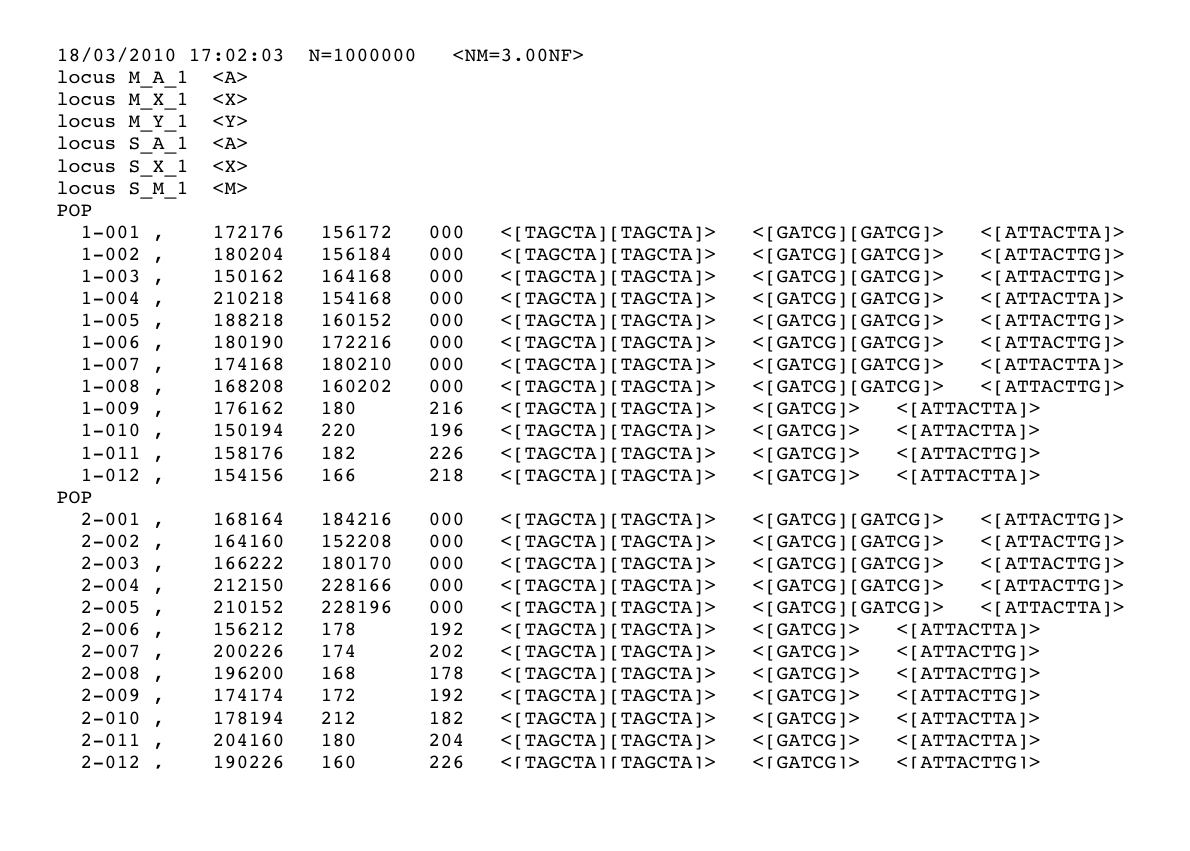
\includegraphics[scale=0.6]{gui_pictures/screenga001.png}
\end{figure}
\newpage
In the second example, the species is haploid. Individuals have been genotyped at three autosomal microsatellite loci and one mitochondrial DNA sequence locus. The species being haploid (deduced from the presence of autosomal haploid loci), no indication of the sex-ratio appears in the title line.

\begin{figure}[h]
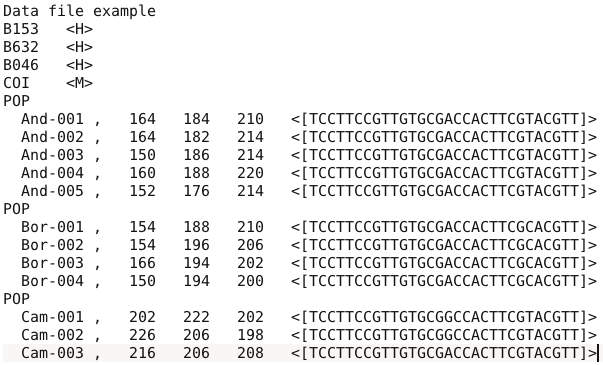
\includegraphics[scale=0.6]{gui_pictures/screenga002.png}
\end{figure}

In the third example, the species is diploid and has been genotyped at a large number of SNP autosomal loci. The first line provides the title which includes the species sex-ratio. The second line indicates what's in the different columns : individual name in column 1, individual sex in column 2, population name in column 3 and one column per SNP locus (the letter \texttt{A} indicates that the autosomal locus is autosomal; it would be \texttt{X} for an X-linked locus, \texttt{Y} for a Y-linked locus and \texttt{M} for a mitochondrial locus) . Columns are sparated by one or more spaces. SNP are coded 0, 1 or 2 according to the number of reference alleles at the corresponding locus. Only the top left part of the data file is represented below :

\begin{figure}[h]
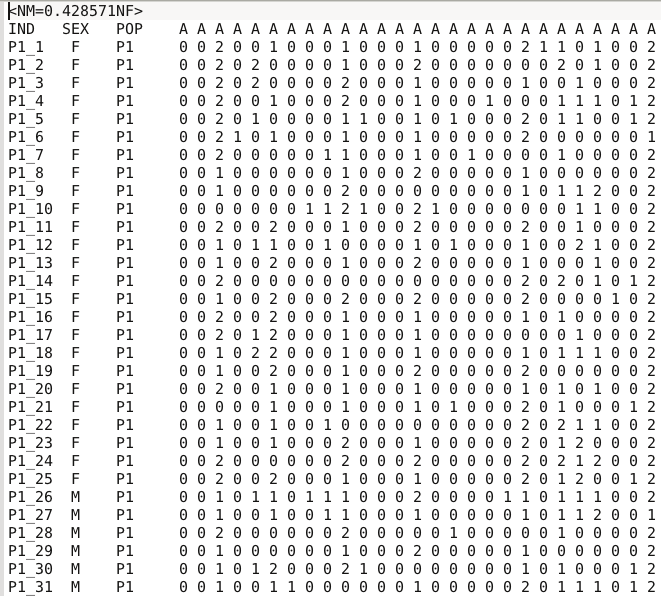
\includegraphics[scale=0.5]{gui_pictures/screenga003.png}
\end{figure}



\clearpage
\section{Cluster version}\label{cluster}
The ABC approach requires simulating data sets, which is a time consuming. Typically, one to several millions data sets are needed to build up a reference table and this process can last several hours to several days. To take advantage of a computer grid cluster, the user can activate the option on the cluster tab of the general settings. By checking \textsf{use a cluster}, the settings of the cluster tab are editable and, while this option remains checked, DIYABC will not compute any reftable on your computer. 

A reftable is generated in 3 sequential steps :
\begin{enumerate}
 \item configure the required parameters in the GUI frontend and generate the cluster bundle (set of zipped files)
 \item transfer the bundle to the cluster and run it
 \item transfer back the reference table and include it to the project
\end{enumerate}

\subsection{configure the required parameters in the GUI frontend and generate the cluster bundle}\label{clusterconfigure}
In the settings cluster tab, you can configure some parameters which will be included in a bash script (cf section 3.7.1). This bash script named \texttt{launch.sh} will be executed on the cluster (cf section \ref{clusterrun}). The bash script is artificially split in two parts in the interface.

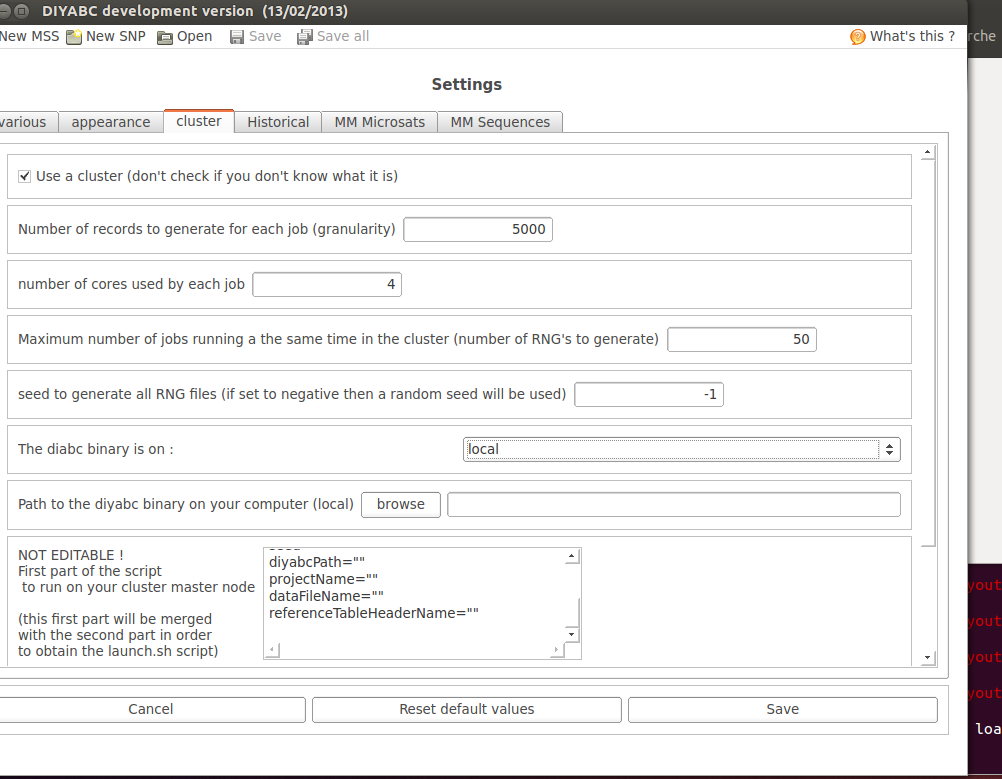
\includegraphics[scale=0.33]{gui_pictures/Capture-DIYABC-cluster.png} \\


You have to understand and edit five parameters of the cluster settings. Each one will be used as a variable in the main script \texttt{launch.sh}.
 

\subsubsection{number of data sets by job}
\texttt{numSimulatedDatasetByJob} : This integer indicates the number of data sets produced by each single job. It represents the granularity of your computations on the cluster. It gives you the hand to optimize your cluster utilization, i.e. the larger \texttt{numSimulatedDatasetByJob}, the less jobs will be created that consume more time. This option enables to optimize your use of the cluster according to your access limitations. The number of jobs submitted on the cluster is given the total number of data sets divided by \texttt{numSimulatedDatasetByJob}. 

A few examples illustrate the importance of this parameter:
\begin{itemize}
 \item  if your cluster is overloaded and the waiting time in queue is long then it is preferable to choose a high amount of data sets by job (less jobs)
 \item if a queue for short jobs is free while the other ones are full then it is preferable to choose a low amount of data sets by job (more jobs) and submit to the short queue
\end{itemize}

\subsubsection{number of cores by job}
\texttt{coresPerJob} : This integer indicates how many CPU cores will be used by each job. Be carefull : if you use lots of cores, to generate the RNG states will be time consuming (fig \ref{fig:rngTimeGeneration}). Increasing the number of cores generally increases the queueing waiting time. Remember that a job with 40 cores will not run faster than 40 jobs with one core each. \\
DIYABC includes openMP. It means that DIYABC can use several cores in a single computer but as it does not include MPI it can not use many cores on many computers for one same job. So please be sure to use an apropriate parallele environment to submit your jobs. Ask to your cluster system administrator. 

\begin{figure}[htb]
\centering \it	
  \begin{tabular}{|  l || c | c | c | c | c | c | c | }
	   \hline
	   number of jobs (t) & \multicolumn{7}{c|}{number of cores (c)} \\
	          & 1 & 4   & 8     & 16 & 32 & 40 & 80 \\
	   \hline \hline
	   100 & 20''  & 1'20" & 3'  & 10'   & 20'   & 26'   & 30' \\
	   \hline
	   200 & 50" & 3'    & 7'  & 20'   & 40'   & 50'   & 1h10' \\
	   \hline
	   500 & 2'  & 8'    & 25' & 50'   & 1h40' & 2h06' & 2h45' \\
	   \hline
	   1000 & 4' & 16'   & 50' & 1h40' & 2h10' & 2h45' & \\
	   \hline
   \end{tabular}
  \caption[width=.6\textwidth]{\label{fig:rngTimeGeneration} \it\footnotesize
    \textbf{RNG files Time Generation.} As shown in section~\ref{rng}, one caveat of the RNG
    method is the obligate generation of all the RNG files at once (generating the RNG files one by one 
    for each job on a cluster is possible but will result in a dangerous bias). The second
    caveat of the RNG method is a consequence of the first one, ie the time needed to generate the RNG
    files increases depending on the number of RNG files \texttt{t} and the number of cores \texttt{c}
    available for each RNG file. Once a file is generated, it is not possible to add cores. }
\end{figure}

\subsubsection{the number of concurrent jobs}
\texttt{maxConcurrentJobs} : This integer indicates the maximum number of jobs allowed to run simultaneously on the cluster. Why is this information required ? One caveat of the RNG (section \ref{rng}) is the need to simultaneously generate all RNG files, before starting the jobs queue submission. The main script \texttt{launch.sh} will produce a pool of RNG files and the script \texttt{nodes.sh} running on each cluster node will randomly draw a RNG file not currently in use. Once again, you should ask your cluster system administrator to know the running jobs limitation on your cluster. You can also evaluate this number by looking at your cluster load. Be carefull : if you use lots of RNG files, to generate the RNG states is time consuming (fig \ref{fig:rngTimeGeneration}).

\subsubsection{the seed to generate RNG files}
\texttt{seed} : This integer indicates to DIYABC the seed to start producing RNG files. By wrinting \texttt{-1} you will ask to use a random seed (recommended). Using a user-defined seed is only for test or debbugging purposes. 

\subsubsection{The diyabc executable}
\texttt{diyabcPath} : This path is for the binary executable to be used on the cluster. There is to way of use it :
\begin{itemize}
 \item  By choosing \texttt{cluster}, you are invited to write the absolute path of a diyabc binary as it match to your cluster file architecture. By this way the script \texttt{node.sh} will know which diyabc cluster binary to use. Ask your cluster administrator in order to know this path. This absolut path need to be the same for all your cluster nodes. 
 \item  By choosing \texttt{local}, you are invited to write the path of a diyabc binary executable on your personal computer. This binary will be added to the bundle to be tranfered to your cluster
\end{itemize}

\subsubsection{main script : launch.sh}
The next two text boxes in the interface deal with the first and last parts of the main script \texttt{launch.sh}. \texttt{launch.sh} will generate a pool of RNG files, submit jobs to the scheduler queuing system using a \texttt{node.sh} script, monitor the jobs and pool all reftable files into a single reftable file when all jobs are completed.

\begin{description}
	\item[first part] This part is not editable as it includes the variables used by DIYABC GUI frontend and other variables from your project : \texttt{numSimulatedDataSet}, \texttt{projectName}, \texttt{dataFileName}. 
	
	\item[last part] This part deals with the jobs submission. By default, \texttt{launch.sh} targets a $Grid Engine$ cluster. You probably need to customise this script to fit your cluster configuration (scheduler system, queue name, ...). You should mainly need to modify the  \texttt{\#\#\#\#\# EDIT \#\#\#\#\#} section. Please ask for help to your cluster system administrator.
\end{description}

\subsection{transfer the bundle to the cluster and run it}\label{clusterrun}
Once you have checked the box \textsf{Use a cluster (...)}, configured the cluster parameters and the \texttt{launch.sh} script in the general settings and saved them, you need to click on the \fbox{\textsf{Run computation}} button from your project panel. Next, you will need to choose a name for a tar archive including all files necessary for the cluster run, and save it on your computer. In order to transfer the tar archive to your cluster account you will probably need an sftp client like FileZilla or WinSCP. Once the archive is stored on your cluster working directory, you will need to login on your cluster with a shell console and untar your archive typing :\\
%\fbox{
   \begin{minipage}{0.9\textwidth}
\begin{lstlisting}
tar -xvf <yourTarArchiveName.tar>
cd yourTarArchiveName

\end{lstlisting}
   \end{minipage}
%}

 This will create a directory with all the files needed to run DIYABC :
\begin{enumerate}
    \item \textsf{general} : the DIYABC executable
    \item \textsf{header.txt} : the header file
    \item \textsf{launch.sh} : the main script to run
    \item \textsf{node.sh} : the script that will be runned by your scheduler for each job
    \item \textsf{$<yourData.mss>$} : the data file 
\end{enumerate}
Now, you have to run the main script \texttt{launch.sh}. \texttt{launch.sh} will run node.sh for each job

\subsubsection{launch.sh}

Once you are in the $<yourTarArchiveName>$ directory, you can run \texttt{launch.sh}. For instance, for a total of 50,000 data sets to be produced through 5 jobs of 10,000 data sets:\\
%\fbox{%
   \begin{minipage}{0.99\textwidth}
 
\definecolor{dkgreen}{rgb}{0,0.6,0}
\definecolor{gray}{rgb}{0.5,0.5,0.5}
\definecolor{mauve}{rgb}{0.58,0,0.82}
 
\lstset{ 
  language=bash,                % the language of the code
  basicstyle=\footnotesize,           % the size of the fonts that are used for the code
  numbers=left,                   % where to put the line-numbers
  numberstyle=\tiny\color{gray},  % the style that is used for the line-numbers
  stepnumber=1,                   % the step between two line-numbers. If it's 1, each line 
                                  % will be numbered
  numbersep=5pt,                  % how far the line-numbers are from the code
  backgroundcolor=\color{white},      % choose the background color. You must add \usepackage{color}
  showspaces=false,               % show spaces adding particular underscores
  showstringspaces=false,         % underline spaces within strings
  showtabs=false,                 % show tabs within strings adding particular underscores
  frame=single,                   % adds a frame around the code
  rulecolor=\color{black},        % if not set, the frame-color may be changed on line-breaks within not-black text (e.g. comments (green here))
  tabsize=4,                      % sets default tabsize to 2 spaces
  captionpos=b,                   % sets the caption-position to bottom
  breaklines=true,                % sets automatic line breaking
  breakatwhitespace=false,        % sets if automatic breaks should only happen at whitespace
  title=\lstname,                   % show the filename of files included with \lstinputlisting;
                                  % also try caption instead of title
  keywordstyle=\color{black},          % keyword style
  commentstyle=\color{dkgreen},       % comment style
  stringstyle=\color{mauve},         % string literal style
  escapeinside={\%*}{*)},            % if you want to add LaTeX within your code
  morekeywords={*},              % if you want to add more keywords to the set
  deletekeywords={}              % if you want to delete keywords from the given language
}


\begin{lstlisting}
>launch.sh
** Generation of RNG files :
./general -p ./ -n "t:1;c:5;s:1038"

** jobs submition :

qsub -N n1_test -q short.q -cwd node.sh 10000 /home/dehneg/DIYABCtest 1  test.mss
Your job 111598 ("n1_test") has been submitted

qsub -N n2_test -q short.q -cwd node.sh 10000 /home/dehneg/DIYABCtest 2  test.mss
Your job 111599 ("n2_test") has been submitted

qsub -N n3_test -q short.q -cwd node.sh 10000 /home/dehneg/DIYABCtest 3  test.mss
Your job 111600 ("n3_test") has been submitted

qsub -N n4_test -q short.q -cwd node.sh 10000 /home/dehneg/DIYABCtest 4  test.mss
Your job 111601 ("n4_test") has been submitted

qsub -N n5_test -q short.q -cwd node.sh 10000 /home/dehneg/DIYABCtest 5  test.mss
Your job 111602 ("n5_test") has been submitted

** monitoring :
0/5 finished 0%  (total : 0)
1/5 finished 20% (total : 10000)
1/5 finished 20% (total : 10000)
2/5 finished 40% (total : 20000)
4/5 finished 80% (total : 40000)
5/5 finished 100% (total : 50000)

** reftables concatenation  :
./general -p /home/dehneg/DIYABCtest -q 2>&1 concat.out
*************************************************************
All the result files have been concatenated into reftable.bin
See concat.out output file for logs
*************************************************************
\end{lstlisting}
   \end{minipage}
%}
\begin{enumerate}
    \item line 3 : generation of all RNG files : \textsf{RNG\_state\_0000.bin}, ..., \textsf{RNG\_state\_0005.bin}
    \item lines 7, 10, 13, 16, 19 : job submission 
    \item lines 23 to 28 : jobs status given every 30 seconds
    \item line 31 : merge all \textsf{reftable\_$<number>$.bin} file in one reftable file \textsf{reftable.bin}. In case of any problem, please read \textsf{concat.out} output file.
\end{enumerate}
Once the monitoring phase starts, you can quit \texttt{launch.sh} and restart it at any time. Since all jobs are submitted by \texttt{launch.sh}, a lock file named \texttt{launch.sh.lock} is written in your $yourTarArchiveName$ directory and inform any new execution of \texttt{launch.sh} to not submit any new job.

\subsubsection{node.sh}
\texttt{node.sh runs} on your cluster nodes for each jobs. Those are the sequential steps of \texttt{node.sh} :
\begin{enumerate}
    \item create a $job id$ name according to the following pattern : \texttt{<node hostname>-n-<sequential number of the job>-pid<pid of nodes.sh execution>-<a random number>} ($pid$ mean Process IDentifier).
    \item Use the scheduler temporary directory if the scheduler provide a \texttt{TMPDIR} environment variable or create a working temporary directory \texttt{/tmp/tmpDiyabc\_<job id>} on the cluster node.
    \item Choose a RNG file from the pool of RNG files created by \texttt{launch.sh}. It means that the node must access your diyabc $yourTarArchiveName$ directory in your working directory. 
    \item As long as \texttt{node.sh} is using the choosen RNG file, you won't see the RNG file in the $yourTarArchiveName$ directory but a lock file named \texttt{<the choosen RNG file name>}.lock and a flag file named the \texttt{<choosen RNG file name>\_<date of the run>\_<job id>}. The flag file contain the local pid of the job on the node of DIYABC. Once DIYABC has finished and updated the RNG file, you will see it again, but not the lock and flag files.
    \item run DIYABC (general file) of course !
    \item copy periodically the reftable log file to the $yourTarArchiveName$ directory. Thus, \texttt{launch.sh} can inform you of the status of the total dataset computed.
\end{enumerate}



\subsection{transfer back the reference table and include it into your computer project}\label{clusterback}
Once your final \texttt{reftable.bin} file has been produced, you need to transfer it from the cluster to you DIYABC project directory on your own computer. Once again, you can use an sftp client.


\clearpage
\subsection{A note about the random number generator used in DIYABC}\label{rng}
By nature, a random number generator (RNG) is a sequential algorithm,
as described in Figure~\ref{fig:rng1} below. Indeed, we shall describe a RNG
by its updating function $f$ changing deterministically the internal
state.  Each time the user requires a new realization of the uniform
distribution over $[0;1)$, the algorithm derives a value $u_k$ from
the current internal state $i_k$ and then updates this state with $f$.
Hence a first and important issue for parallel Monte Carlo
computations is to design independent RNGs that might run in parallel
while minimizing the communications between processors. It is quite
standard to use as many RNGs as computing cores in the computer or in
the cluster of computers. 


\begin{figure}[htb]
\centering \it
\begin{minipage}[c]{.6\linewidth}
  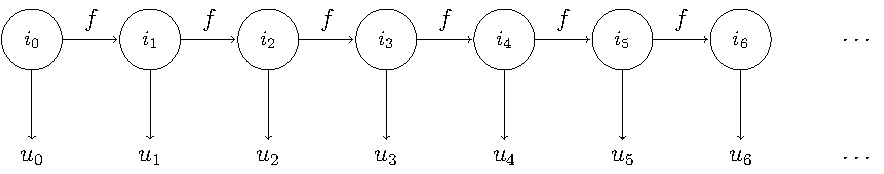
\includegraphics[width=\textwidth]{DCMT_rng.pdf}
  \caption[width=.6\textwidth]{\label{fig:rng1} \it\footnotesize
    \textbf{Random Number Generator.} A RNG is an algorithm
    that produces a sequence
    of floating numbers, says $u_0, u_1, \ldots$, that resembles a
    sequence of independant random numbers, uniformly distributed over
    $[0;1)$.
    It uses a sequence of
    internal states, say $i_0, i_1,\ldots$, which are computed by
    reccurence, namely, $i_{k+1}=f(i_k)$. The first internal state
    $i_0$ is often named the seed.}
\end{minipage}
\end{figure}

The second
version of DIYABC uses the Dynamic Creator (DCMT) of
\citet{DCMT} to look for a set of independent
Mersenne-Twister generators. Actually, the updating function $f$ of a
Mersenne-Twister generator is parametrized by a few integer
numbers. 
The output of the DCMT is a set of $N$ updating functions,
say $\{f^{(1)}, \ldots, f^{(N)}\}$, producing independent streams. 
That is, the $n$-th RNG is a sequence of iternal states
$i_0^{(n)},i_1^{(n)}, i_2^{(n)}, \ldots$ satisfying
$i_{k+1}^{(n)}=f^{(n)}(i_k^{(n)})$
that gives rise to a sequence of independent, uniformly distributed numbers
$u_0^{(n)}, u_1^{(n)}, u_2^{(n)},\ldots$.
We found that the DCMT was simple to use and gave good results.  There
is no limitation on the number $N$ of RNGs it produces. Once initialized,
the different RNGs do not require any communication between them and
each of them runs as quickly as a single Mersenne-Twister
generator. But an important limitation is that it is impossible to add a
new RNG to the set produced by the DCMT. Practically, this means that
we have to know \textit{a priori} a bound on the number of
jobs working together in parallel. See XXX Alex XXX.





%%% Local Variables: 
%%% mode: latex
%%% TeX-master: "Notice_DIYABC_principal"
%%% End: 



  

\begin{thebibliography}{a}
\bibitem[Beaumont \emph{et al.}, 2002]{B2002} Beaumont, M. A., W. Zhang and D. J. Balding, 2002. Approximate Bayesian Computation in Population Genetics. \emph{Genetics} \textbf{162}, 2025-2035.
\bibitem[Beaumont, 2008]{B2008}Beaumont, M.A., 2008. Joint determination of topology, divergence time, and immigration in population trees. In Simulation, Genetics, and Human Prehistory, eds. S. Matsumura, P. Forster,  C. Renfrew. McDonald Institute Press, University of Cambridge (\emph{in press}).
\bibitem[Begg and Gray, 1984]{BG1984} Begg, C.B. and R. Gray, 1984. Calculation of polychotomous logistic regression parameters using individualized regressions. \emph{Biometrika},
\textbf{71}, 11-18.
\bibitem[Belkhir \emph{et al.}, 1996-2004]{BB1996} Belkhir K., Borsa P., Chikhi L., Raufaste N. and F. Bonhomme, 1996-2004 GENETIX 4.05, logiciel sous Windows TM pour la g�n�tique des populations. Laboratoire G�nome, Populations, Interactions, CNRS UMR 5171, Universit� de Montpellier II, Montpellier (France).
\bibitem[Bertorelle and Excoffier, 1998]{BE1998} Bertorelle, G. and L. Excoffier, 1998. Inferring admixture proportion from molecular data. \emph{Mol. Biol. Evol.} \textbf{15}, 1298-1311.
\bibitem[Choisy  \emph{et al.}, 2004]{CF2004} Choisy, M., P. Franck and J.M. Cornuet, 2004. Estimating admixture proportions with microsatellites : comparison of methods based on simulated data. \emph{Mol. Ecol.} \textbf{13}, 955-968.
\bibitem[Chakraborty and Jin, 1993]{CJ1993}Chakraborty R and L Jin, 1993. A unified approach to study hypervariable polymorphisms: statistical considerations of determining relatedness and population distances. EXS. \emph{67}, 153�175.
\bibitem[Cornuet \emph{et al.}, 2006]{C2006} Cornuet, J. M.,
M. A. Beaumont, A. Estoup and M. Solignac, 2006. Inference on
microsatellite mutation processes in the invasive mite, \emph{Varroa
destructor}, using reversible jump Markov chain Monte Carlo.
\emph{Theoret. Pop. Biol.} \textbf{69}, 129-144.
\bibitem[Cornuet \emph{et al.}, 2010]{C2010}Cornuet J.M., V. Ravign\'e and A. Estoup, 2010. Inference on population history and model checking using DNA sequence and microsatellite data with the sofware DIYABC (v1.0). \emph{submitted}. 
\bibitem[Cornuet \emph{et al.}, 2008]{C2008}Cornuet J.M., F. Santos, M.A. Beaumont, C.P. Robert, J.M. Marin, D.J. Balding, T. Guillemaud and A. Estoup, 2008. Infering population history with DIYABC: a user-friendly approach to Approximate Bayesian Computations. \emph{Bioinformatics}, \textbf{24} (23), 2713-2719.

\bibitem[Estoup \emph{et al.}, 1993]{E1993} Estoup, A., M. Solignac, M. Harry and J.M. Cornuet, 1993. Characterization of $(GT)_n$ and $(CT)_n$ microsatellites in two insect species: \emph{Apis mellifera} and \emph{Bombus terrestris}. \emph{Nucl. Ac. Res.}, \textbf{21}, 1427-1431.
\bibitem[Estoup \emph{et al.}, 2001]{E2001} Estoup, A., I. J. Wilson, C. Sullivan, J. M. Cornuet and C. Moritz, 2001 Inferring population history from microsatellite et enzyme data in serially introduced cane toads, \emph{Bufo marinus}. \emph{Genetics}, \textbf{159}, 1671-1687.
\bibitem[Estoup \emph{et al.}, 2002]{E2002}Estoup, A., P. Jarne and J.M. Cornuet, 2002.
 Homoplasy and mutation model at microsatellite loci and their consequences for population
 genetics analysis. \emph{Mol. Ecol.}, \textbf{11}, 1591-1604.
\bibitem[Estoup and Clegg, 2003]{EC2003} Estoup, A. and S. M. Clegg, 2003. Bayesian inferences on the recent islet colonization history by the bird Zosterops lateralis lateralis. \emph{Mol. Ecol.} \textbf{12}: 657-674.
\bibitem[Estoup \emph{et al.}, 2004]{EB2004}Estoup, A., M.A. Beaumont, F. Sennedot, C. Moritz and J.M. Cornuet, 2004. Genetic analysis of complex demographic scenarios : spatially expanding populations of the cane toad, \emph{Bufo marinus}. \emph{Evolution},\textbf{58}, 2021-2036.
\bibitem[Estoup \emph{et al.}, 2012]{EL2012}Estoup, A., E. Lombaert, J.M. Marin, T. Guillemaud, P. Pudlo, C.P. Robert and J.M. Cornuet, 2012. Estimation of demo-genetic model probabilities with Approximate Bayesian Computation using linear discriminant analysis on summary statistics. \emph{Molecular Ecology Resources}, \textbf{12}, 846-855.

\bibitem[Excoffier \emph{et al.}, 2005]{Ex2005} Excoffier, L., A. Estoup and J.M. Cornuet, 2005.
 Bayesian analysis of an admixture model with mutations and arbitrarily linked markers. \emph{Genetics} \textbf{169}, 1727-1738.
\bibitem[Fagundes \emph{et al.}, 2007]{FR2007} \textsc{Fagundes, N.J.R., N. Ray, M.A. Beaumont, S. Neuenschwander, F. Salzano, S.L. Bonatto and L. Excoffier}, 2007. Statistical evaluation of alternative models of human evolution. \emph{Proc. Natl. Acad. Sc.}, \textbf{104} : 17614-17619.
\bibitem[Fu and Chakraborty, 1998]{F1998} Fu, Y.X. and
Chakraborty, R., 1998. Simultaneous estimation of all the parameters
of a stepwise mutation model. \emph{Genetics}, \textbf{150},
487-497.
\bibitem[Garza and Williamson, 2001]{GW2001} Garza JC and E Williamson, 2001. Detection of reduction in population size using data from microsatellite DNA. \emph{Mol. Ecol.}   \textbf{10},305-318.
\bibitem[Gelman \emph{et al.}, 1995]{GCSR1995} Gelman, A., J.B. Carlin, H.S. Stern and D.B. Rubin, 1995. \emph{Bayesian Data Analysis}. Chapman et Hall, London, 526p. 
\bibitem[Golstein \emph{et al.}, 1995]{GL1995} Goldstein DB, Linares AR, Cavalli-Sforza LL, and Feldman MW, 1995. An evaluation of genetic distances for use with microsatellite loci. \emph{Genetics} \textbf{139}, 463-471.
 \bibitem[Goudet, 1995]{G1995} Goudet, J. ,1995. FSTAT (Version 1.2): A computer program to calculate F- statistics. \emph{J. Hered.} \textbf{86},  485-486.
 \bibitem[Griffiths and Tavar\'e, 1994]{GT1994} Griffiths, R.C. and S. Tavar\'e, 1994. Simulating probability distributions in the coalescent. \emph{Theor. Pop. Biol.} \textbf{46}, 131-159.
\bibitem[Guillemaud  \emph{et al.}, 2010]{G2010}Guillemaud T., M.A. Beaumont, M. Ciosi, J.M. Cornuet and A. Estoup, 2010. Inferring introduction routes of invasive species using approximate Bayesian computation on microsatellite data. \emph{Heredity}, \textbf{104}, 88-99.
\bibitem[Haag-Liautard \emph{et al.}, 2008]{HL2008} Haag-Liautard C., N. Coffey, D. Houle, M. Lynch, B. Charlesworth and P.D. Keightley, 2008. Direct estimation of the mitochondrial DNA mutation rate in Drosophila melanogaster. \emph{Plos Biol}, \textbf{6}, e204.
 \bibitem[Hamilton \emph{et al.}, 2005]{HS2005} Hamilton, G., M. Stoneking and L. Excoffier, 2005. Molecular analysis reveals tighter social regulation of immigration in patrilocal populations than in matrilocal populations. \emph{Proc. Natl. Acad. Sci. USA}, \textbf{102}, 7476-7480.
\bibitem[Hasegawa  \emph{et al.}, 1985]{HKY1985} Hasegawa, M., Kishino, H and Yano, T., 1985. Dating the human-ape splitting by a molecular clock of mitochondrial DNA. \emph{Journal of Molecular Evolution} 22:160-174.
\bibitem[Hudson \emph{et al.}, 1992]{H1992} Hudson,R. R., M. Slatkin and W.P. Maddison, 1992. Estimation of levels of gene flow fom DNA sequence data. \emph{Genetics}, 132, 583-589.
\bibitem[Ihaka and Gentleman, 1996]{IG1996}Ihaka R. and R. Gentleman, 1996. $R$: a language for data analysis and graphics. \emph{J.  Comput. Graph. Stat.}, \textbf{5}, 299-314
\bibitem[Ingvarsson, 2008]{I2008} Ingvarsson P.K., 2008. Multilocus patterns of nucleotide polymorphism and the demographic history of \emph{Populus tremula. Genetics}, 180: 329-340.
\bibitem[Jukes and Cantor, 1969]{JK1969}Jukes, TH and Cantor, CR., 1969. Evolution of protein molecules. Pp. 21-123 in H. N. Munro, ed. \emph{Mammalian protein metabolism}. Academic Press, New York.
\bibitem[Kimura, 1980]{K1980}Kimura, M., 1980. A simple method for estimating evolutionary rate of base substitution through comparative studies of nucleotide sequences. \emph{Journal of Molecular Evolution} 16:111-120.
\bibitem[Lombaert \emph{et al.}, 2010]{L2010}Lombaert E., T. Guillemaud, J.M. Cornuet, T. Malausa, B. Facon and A. Estoup, 2010.  Bridgehead effect in the worldwide invasion of the biocontrol harlequin ladybird. \emph{PLoS ONE}, http://dx.plos.org/10.1371/journal.pone.0009743.
\bibitem[Matsumoto and Nishimura, 2000]{DCMT} Matsumoto M and T Nishimura, 2000. Dynamic Creation of Pseudorandom Number Generators. \emph{Monte Carlo and Quasi-Monte Carlo Methods 1998}, Springer, pp 56--69.
\bibitem[Miller \emph{et al.}, 2005]{ME2005} Miller N, A. Estoup, S. Toepfer, D Bourguet, L. Lapchin, S. Derridj, K.S. Kim, P Reynaud, F. Furlan and T. Guillemaud,  2005. Multiple Transatlantic Introductions of the Western Corn Rootworm. \emph{Science}, \textbf{310}, p. 992
\bibitem[Nei, 1972]{N1972} Nei M., 1972. Genetic distance between populations. \emph{Am. Nat.} 106:283-292
\bibitem[Nei, 1987]{N1987} Nei M., 1987. \emph{Molecular Evolutionary Genetics}. Columbia University Press, New York, 512 pp.
\bibitem[Ohta and Kimura, 1973]{O1973} Ohta, T. and Kimura, M.,
1973. A model of mutation appropriate to estimate the number of
electrophoretically detectable alleles in a finite population.
\bibitem[Pascual \emph{et al.}, 2007]{PC2007}Pascual, M., M.P. Chapuis, F. Mestres, J. Balany\'a, R.B. Huey, G.W. Gilchrist, L. Serra and A. Estoup, 2007. Introduction history of \emph{Drosophila subobscura} in the New World : a microsatellite based survey using ABC methods. \emph{Mol. Ecol.}, \textbf{16}, 3069-3083.
\bibitem[Pollock \emph{et al.}, 1998]{PDD1998}Pollock DD, Bergman A, Feldman MW, Goldstein DB, 1998. Microsatellite behavior with range constraints: parameter
estimation and improved distances for use in phylogenetic reconstruction. \emph{Theoretical Population Biology}, \textbf{53}, 256–271.
\bibitem[Pritchard \emph{et al.}, 1999]{P1999} Pritchard, J., M. Seielstad,
A. Perez-Lezaun and M. Feldman, 1999. Population growth of human Y
chromosomes: a study of Y chromosome microsatellites. \emph{Mol.
Biol. Evol.} \textbf{16}, 1791-1798.
\bibitem[Rannala and Moutain, 1997]{RM1997}Rannala, B., and J. L. Mountain, 1997. Detecting immigration by using multilocus genotypes. \emph{Pro. Nat. Acad. Sci. USA} \textbf{94}, 9197-9201.
\bibitem[Raymond and Rousset, 1995]{RR1995} Raymond M., and F. Rousset, 1995. Genepop (version 1.2), population genetics software for exact tests and ecumenicism. \emph{J. Hered.}, \textbf{86}, 248-249
\bibitem[Schug  \emph{et al.}, 1997]{SMA1997} Schug M.D., T.F. Mackay and C.F. Aquadro, 1997. Low mutation rates of microsatellite loci in \emph{Drosophila melanogaster}. \emph{Nat Genet.} \textbf{15}, 99-102.
\bibitem[Stephens and Donnelly, 2000]{SD2000} Stephens, M. and P. Donnelly,
 2000, Inference in molecular population genetics (with discussion).
 J. R. Stat. Soc. B \textbf{62}, 605-655.
 \bibitem[Tajima, 1989]{TA1989}Tajima, F., 1989. Statistical method for testing the neutral mutationhypothesis by DNA polymorphism. \emph{Genetics} 
123: 585-595
 \bibitem[Tamura and Nei, 1993]{TN1993} Tamura, K., and M. Nei., 1993. Estimation of the number of nucleotide substitutions in the control region of mitochondrial DNA in humans and chimpanzees. \emph{Molecular Biology and Evolution} 10:512-526.
\bibitem[V\'azquez  \emph{et al.}, 2000]{VPAD2000} V\'azquez F.J., T. P�rez, J. Albornoz and A. Dom\'inguez, 2000.Estimation of microsatellite mutation rates in \emph{Drosophila melanogaster}. \emph{Genet Res.}, \textbf{76}, 323-6.
\bibitem[Weir and Cockerham, 1984]{WC1984}Weir BS and CC Cockerham , 1984. Estimating F-statistics for the analysis of population structure. \emph{Evolution} \textbf{38}: 1358-1370.
\bibitem[Whittaker \emph{et al.},
2003]{W2003} Whittaker, J.C., Harbord, R.M., Boxall, N., Mackay, I.,
Dawson, G. and Sibly, R.M. 2003. Likelihood-based estimation of
microsatellite mutation rates, \emph{Genetics}, \textbf{164},
781-787.
\end{thebibliography}

\end{document}
